\documentclass[12pt]{article}

\usepackage{times,fullpage,xspace,fancyhdr,url}
\usepackage[pdftex]{graphicx}
\usepackage[pdftex,
            a4paper,
            colorlinks=true,
            urlcolor=black,
            linkcolor=black,
            citecolor=black,
            bookmarksopen=false,
            bookmarksnumbered=true,
            pdfstartview=FitH]{hyperref}

\usepackage{graphicx}
\usepackage{xspace,color}
\pdfcompresslevel=9
\newcommand{\leaguename}{RoboCup Standard Platform League (NAO) }
\hypersetup{
 pdftitle={\leaguename Rule Book},
 pdfauthor={Technical Committee},
}
\usepackage[latin1]{inputenc}
\usepackage{amsmath}

% comment 'disable' in to disable all the todo notes :)
\usepackage
[
%disable
]{todonotes}

\sloppy
\newcommand{\ie}{\mbox{i.\,e.}\xspace}
\newcommand{\eg}{\mbox{e.\,g.}\xspace}
\newcommand{\cf}{\mbox{cf.}\xspace}
\newcommand{\comment}[1]{\marginpar{\pdfannot width 4in height .5in depth 8pt {/Subtype /Text /Contents (#1)}}}
\newcommand{\inparagraph}[1]{\paragraph{#1\hspace{-1em} }}


% some colors
\definecolor{orange}{rgb}{1,0.5,0}
\definecolor{red}{rgb}{1,0,0}
\definecolor{green}{rgb}{0,1,0}


\title{\leaguename Rule Book}
\author{RoboCup Technical Committee}
\date{(Preliminary 2017 rules, as of \today)}

\setlength{\parindent}{0pt}
\setlength{\parskip}{12pt plus 6pt minus 3 pt}
\setcounter{tocdepth}{1}
\widowpenalty=10000
\clubpenalty=10000

\pagestyle{fancy}
\lhead{}
\chead{}
\rhead{}
\lfoot{}
\cfoot{}
\rfoot{}

\renewcommand{\headrulewidth}{0.4pt}
\renewcommand{\footrulewidth}{0.4pt}

\newcommand{\TotalWidth}{7.4~m\xspace}
\newcommand{\TotalLength}{10.4~m\xspace }
\newcommand{\KickOffAutoTime}{45 seconds\xspace}

% needed to align an image and text correctly side by side
\newcommand{\imagebox}[1]{\raisebox{2ex}{\raisebox{-\height}{#1}}}

\begin{document}

\maketitle

\begin{center}
Questions or comments on these rules should be mailed to \url{rc-spl-tc@lists.robocup.org}.
\end{center}

\vfill

\tableofcontents
\setcounter{tocdepth}{3}

\thispagestyle{fancy}

\clearpage

\cfoot{\thepage}
\setcounter{page}{1}

\newpage

\section{Setup of the Environment}

\subsection{Field Construction}
\label{sec:field_dim}

The soccer field consists of 8mm artificial turf mounted on a flat wooden base with a total area of length \TotalLength and width \TotalWidth.  Care should be taken to ensure the field is as flat and level as possible.  Additionally, the wooden base should be well supported and should not give when humans stand or walk on it.

The dimensions of the soccer field are shown in Figure~\ref{fig:field_dim}. Note that the penalty cross is a cross and there is a dash at center field. White field lines should be made of the same 8mm artificial turf, but in white (i.e., made of white artificial turf and not painted).

The construction and placement of the goals is depicted in Figure~\ref{fig:goal_dimensions} and Figure~\ref{fig:goal_appearance}. The support structure for the net shall be made with small black, white, or gray bars or cylinders.  The support structure shall be constructed exactly as shown in Figure \ref{fig:goal_appearance}.


\begin{figure}[b!]
\centerline{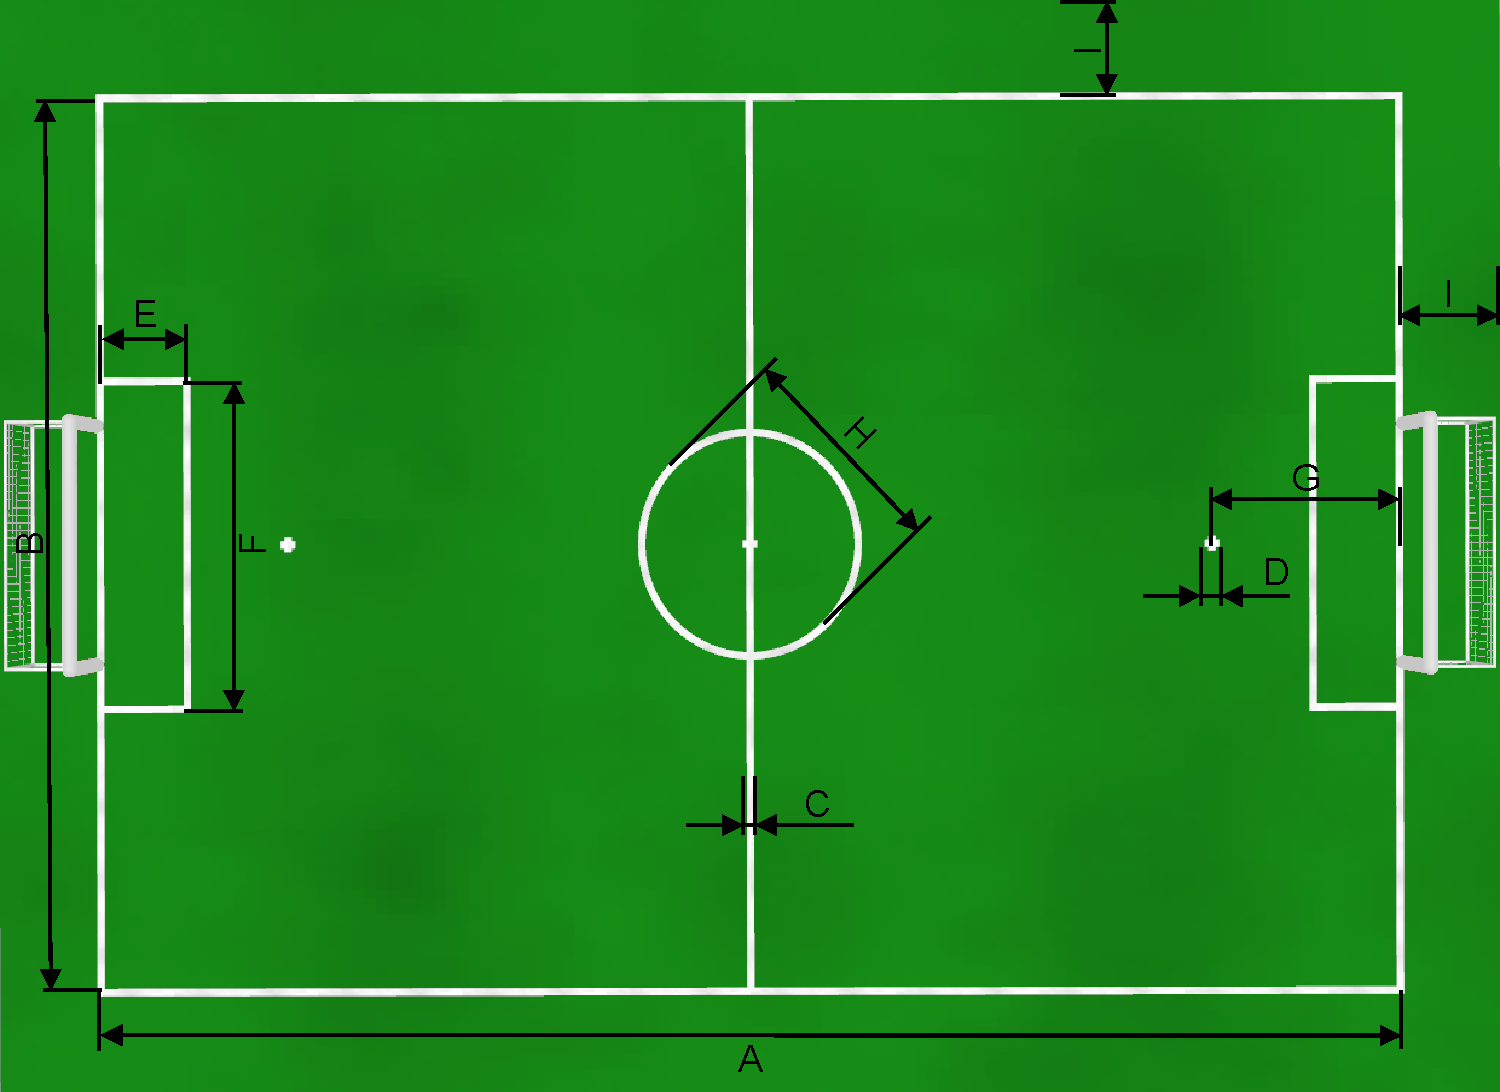
\includegraphics[width=\columnwidth]{figs/fieldDimensions2015.pdf}}
\vspace{1ex}
\begin{tabular}{| l | l | l |}
ID & Description & Length (in mm) \\
\hline
A & Field length & 9000 \\
\hline
B & Field width & 6000 \\
\hline
C & Line width & 50 \\ 
\hline
D & Penalty cross size & 100 \\ 
\hline
 &  &  \\
\end{tabular}
\begin{tabular}{|l|l|l|}
ID & Description & Length (in mm) \\
\hline
E & Penalty area length & 600 \\
\hline
F & Penalty area width & 2200 \\
\hline
G & Penalty cross distance & 1300 \\ 
\hline
H & Center circle diameter & 1500 \\
\hline
I & Border strip width & 700 \\
\end{tabular}
\caption{Schematic diagram of the soccer field (not to scale) and corresponding dimensions in mm.  Note that measurements on this diagram are made to the center of lines.} \label{fig:field_dim}
\end{figure}


\begin{figure}[t!]
\begin{center}
\leavevmode
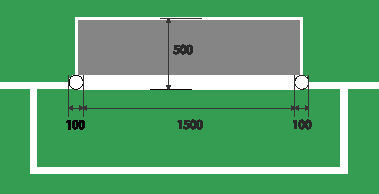
\includegraphics[width=1\columnwidth]{figs/goalDimensions2015.pdf}
\caption{Dimensions of the goal (in mm), viewed from above, and its placement on the field.}
\label{fig:goal_dimensions}
\end{center}
\end{figure}

\begin{figure}[h!]
\begin{center}
\leavevmode
\begin{minipage}[t]{0.49\columnwidth}
\imagebox{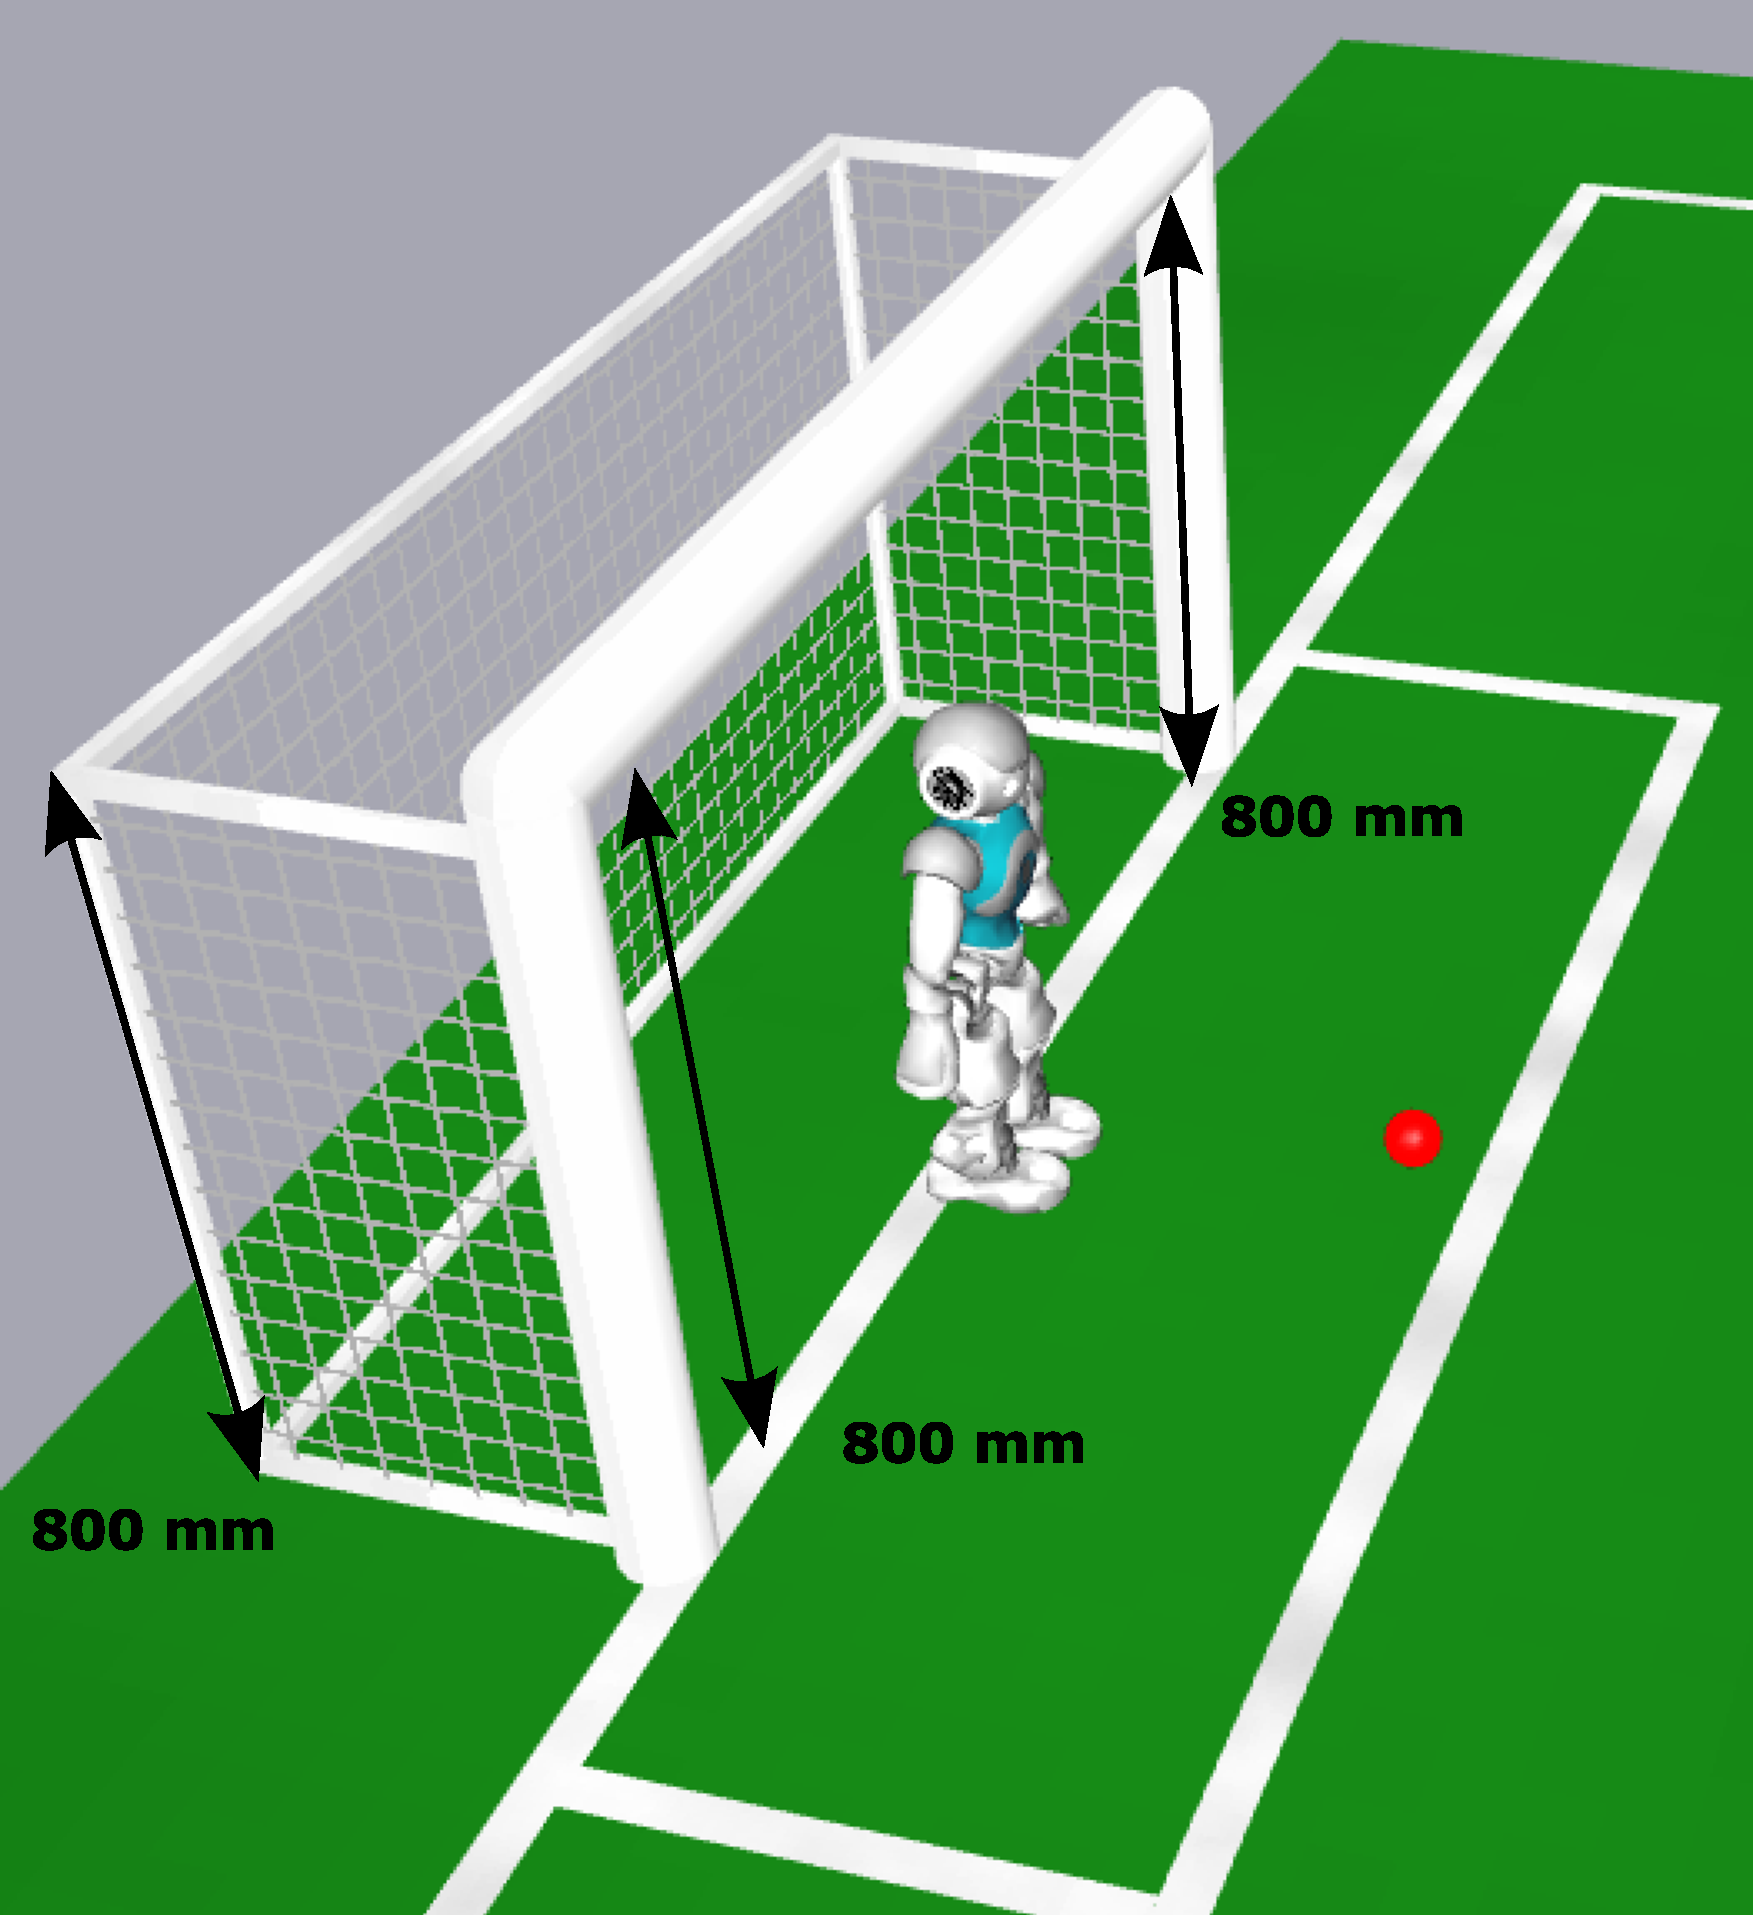
\includegraphics[width=1\columnwidth]{figs/goalDimensions3D.pdf}}%
\end{minipage}
\begin{minipage}[t]{0.49\columnwidth}
The goalposts and crossbar are made from 3 white cylinders with a diameter of 100 mm. 
The net:
\begin{itemize}
\item has a height of 800 mm
\item is of white, gray or black color
\item is tightly supported via the support structure, in a way to minimize interference with the goal keeper
\item has a weave with holes smaller than the ball diameter.
\end{itemize}
\end{minipage}
\caption{Appearance and dimensions of the goals.}
\label{fig:goal_appearance}
\end{center}
\end{figure}

\subsection{Field Colors}

The colors of the soccer field are shown in Figure~\ref{fig:field_color}. All items on the RoboCup field are color-coded:

\begin{itemize}

\item The field (artificial turf) itself is green (color is not specified, but it should not be too dark).

\item The lines on the field are white. They should be made from white artificial turf.

\item Goals~(\cf Figure~\ref{fig:goal_appearance}). The posts and top cross bar of both goals are white. The net and the support structure for the net are white, gray, or black.

\end{itemize}

\begin{figure}[t]
\centerline{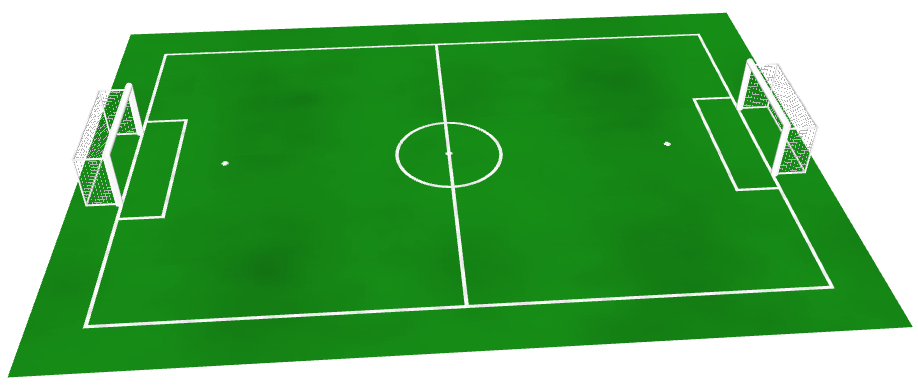
\includegraphics[width=\columnwidth]{figs/emptyfield_2015.png}}
\caption{Field colors and layout.}
\label{fig:field_color}
\end{figure}

\subsection{Lighting Conditions}
\label{sec:lightConditions}
The lighting conditions depend on the actual competition site. As the league moves towards natural lighting conditions, SPL fields will be placed near or under windows where possible. Whether or not window lighting is used, ceiling lights will be provided as necessary to ensure that most of the field is never darker than 300 Lux (400 Lux preferred) during competition venue opening hours. Local organizers should discuss with the technical committee if additional lighting will be needed to meet the minimum lighting requirements.

Lighting is not required to be even and hotspots may occur on the fields. The lighting design (comprising both natural and artificial light sources) shall aim to limit the lighting ratio between the brightest and darkest patches on the field to less than 10 : 1. In general, lighting irregularities, including changes that occur during the competition, are acceptable and will not be cause for delay.  Such irregularities may include sun streaming through windows, light bulbs turning off, light bulbs being replaced, etc.

\subsection{Venue Setup}
\label{sec:boundaries}
Fields may be located close to one another.  Barriers will not necessarily be constructed between adjacent fields to block the robots from seeing other fields, goals, or balls.  However, barriers will be constructed to block sight between any fields that are not located at least three meters apart.  Hence, for each side of a field that is adjacent to another field, either barriers will separate the fields or at least three meters will be between the carpet of adjacent fields.

\subsection{Ball}
\label{sec:ball}

The official ball is a soft foam ball with a black and white soccer ball print (see Figure \ref{fig:ball}). They are 100 mm in diameter and weigh 44 grams. These balls are available by writing to info@sportpaint.de (in German or English) and asking to order the "pu schaumstoffball 10cm 100ss".  Each ball costs EUR 2.50 plus shipping, where shipping cost depends on the destination.

\begin{figure}[t]
  \centerline{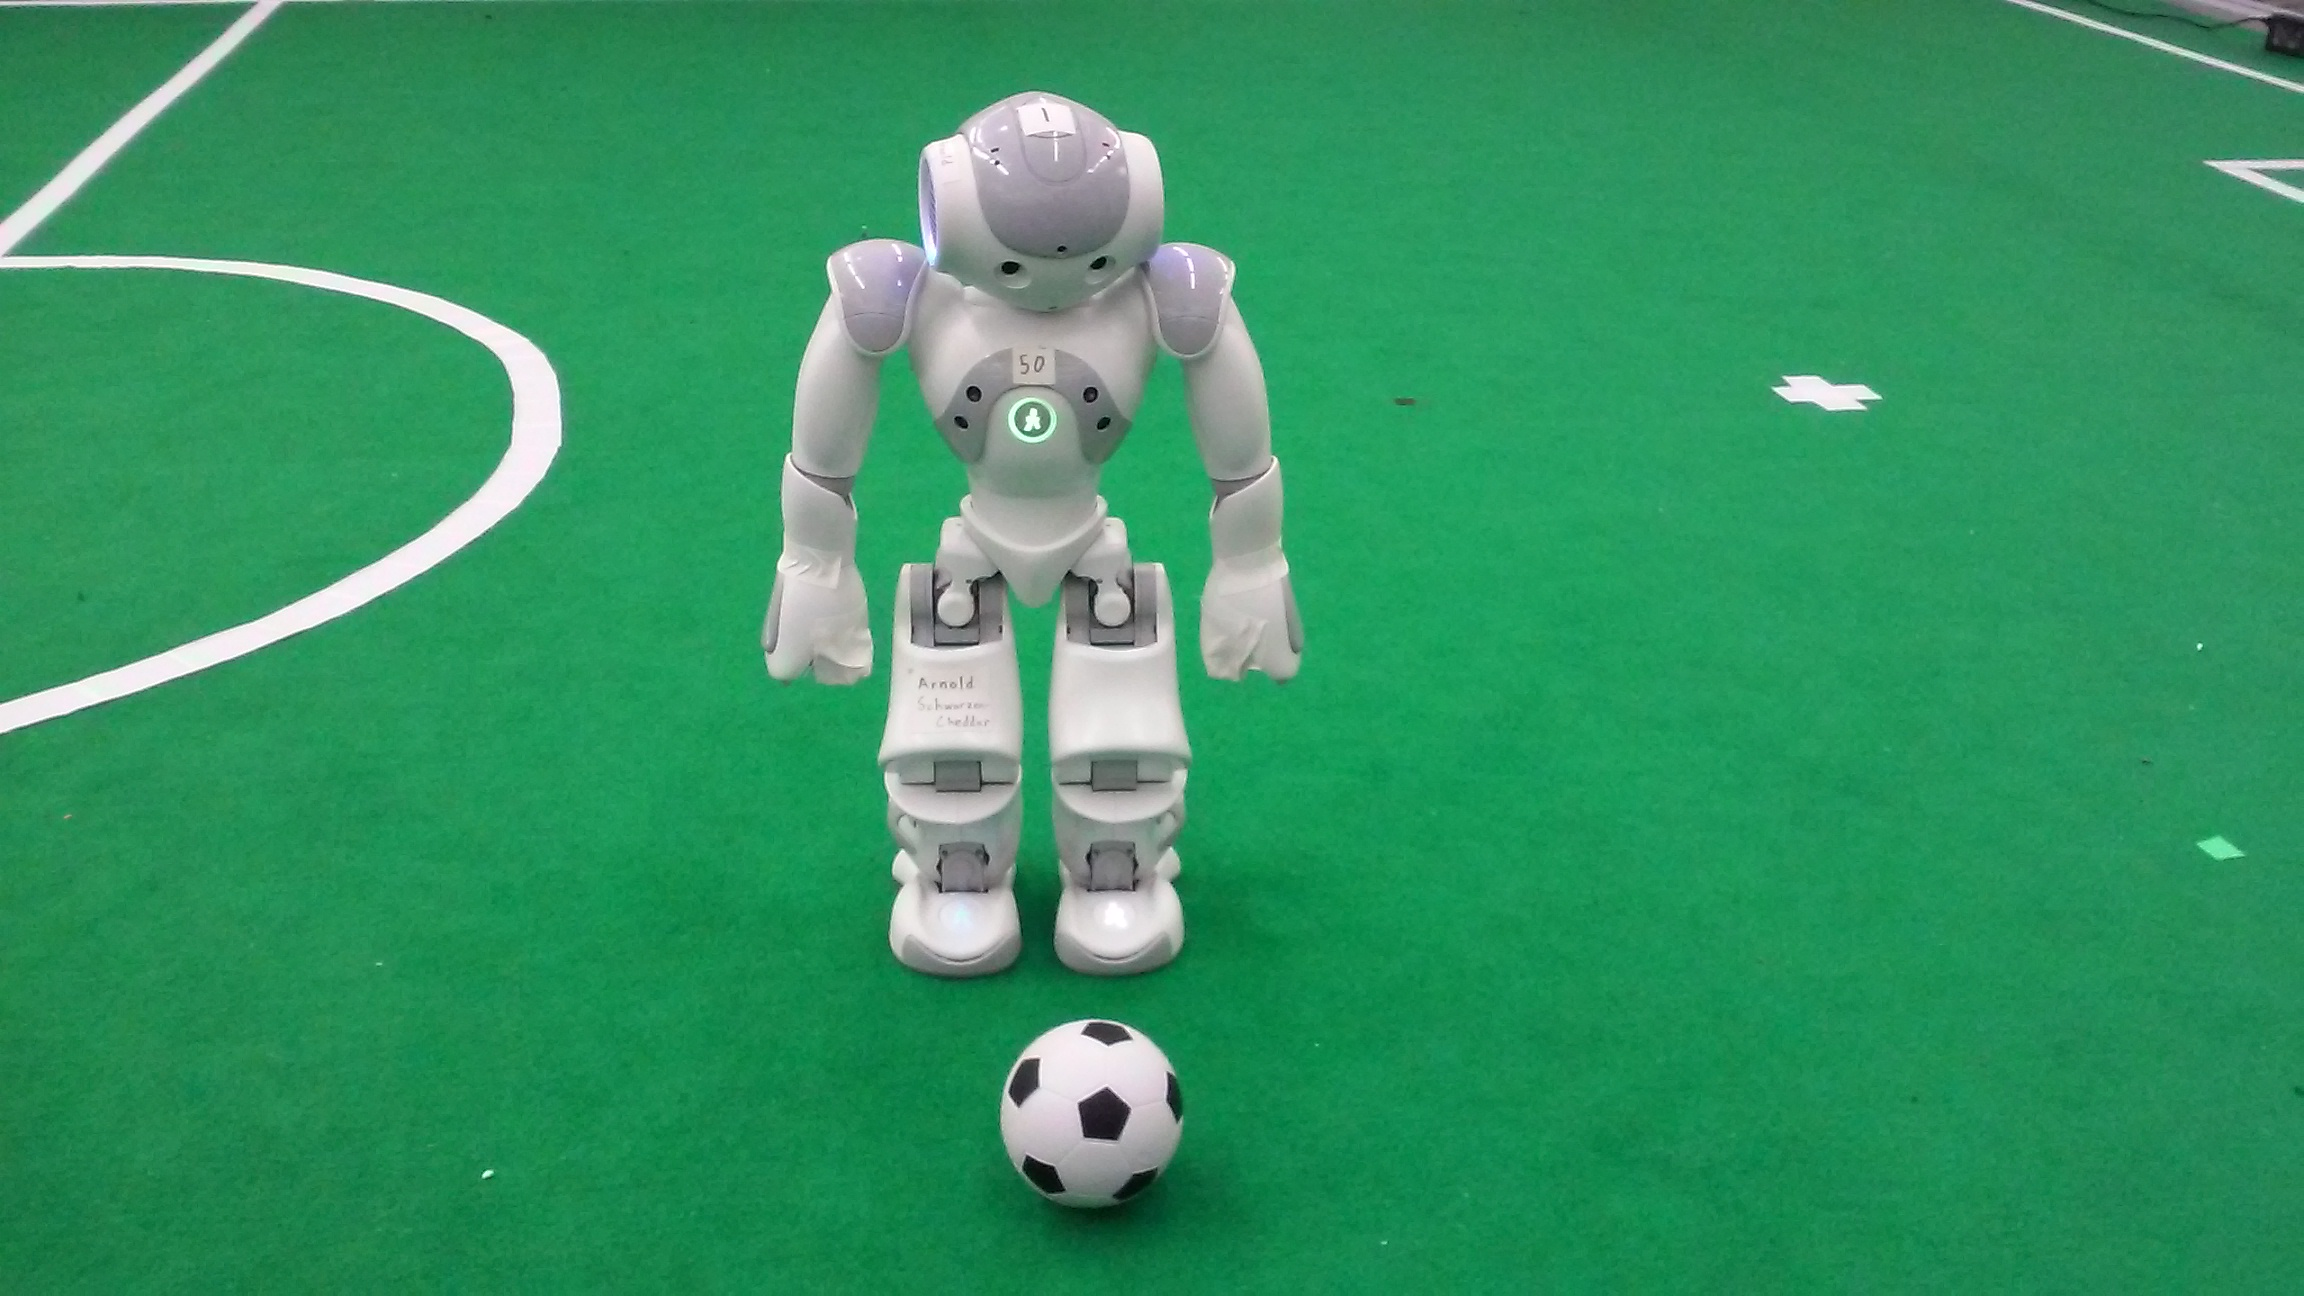
\includegraphics[height=0.28\columnwidth]{figs/robotWithBall2016.jpg}}
  \caption{A NAO and the official ball.}
  \label{fig:ball}
\end{figure}

\newpage


\section{Robot Players}
\label{sec:robot_players}
A match is played by two teams, each consisting of not more than \textbf{5} players and a coaching robot. At most one player may be designated as \emph{goalkeeper}, the others are all \emph{field players}.

\subsection{Hardware}
\label{sec:hardware}
All teams must use gray, red, blue, or orange plated NAO humanoid robots manufactured by SoftBank Robotics. 

Absolutely no modifications or additions to the robot hardware are allowed. No additional hardware is permitted including off-board sensing or processing systems. Additional sensors besides those originally installed on the robots are likewise not allowed. The only exceptions are:

\begin{itemize}

\item Setting the passive wrist joints to a fixed position either with glue or a transparent or white duct tape.

\item Protecting the fingers with white finger protectors provided by the manufacturer or with transparent or white duct tape.

\item For NAO versions that require a memory stick to remain in the head during operation, alternate memory sticks may be used instead of the manufacturer supplied memory sticks.

\end{itemize}

A computer will be provided by the event organizers for the purpose of sending GameController messages to the robots.

\subsection{Goal Keeper}
\label{sec:goal_keeper}

The goal keeper is allowed to touch the ball with its arms/hands only while it is within its own penalty area. It always has the jersey number ``1''.

\subsection{Field Players}
\label{sec:field_players}
Only one field player may enter their own penalty area at any given time. Each of the four field players has a jersey number from the set $\{2, 3, 4, 5, 6\}$. However, by default, the number ``6'' should only be used for a substitute that enters the game later.

\subsection{Coaching Robot}
\label{sec:coaching_robot}

The purpose of the coaching robot is to observe the game from an external position and to give tactical and strategic advice to its team's field players. This is realized by sending messages via a dedicated GameController interface (\cf Section \ref{sec:wireless}). The coaching robot may not communicate via any other mechanism.  A coach is not directly connected to its teammates and should not serve as a remote controller or external vision system.

The coaching robot is not placed on the field but on a table on the same side of the field as the GameController computer.  The coaching robot must be connected via a cable to the GameController. The coaching robot may sit or kneel on the table or in a seat. For safety reasons, it is not allowed to move (except its head and arms --- see \cf Section \ref{sec:coach_motion}) or to enter a pose different from ordinary seating as depicted in Fig. \ref{fig:coaches}.  Seats will not be provided by the organizers, but teams may bring their own seats or small platforms that have a maximum height of the seating surface of 15 cm. Except for a backrest that is not higher than the sitting robot, no additional elements such as flags are allowed to be attached to the seats. Teams may position the coach anywhere they wishon a table on the same side of the field as the GameController computer.  The coach may only be moved at half-time and during time-outs.

\begin{figure}[t]
  \centerline{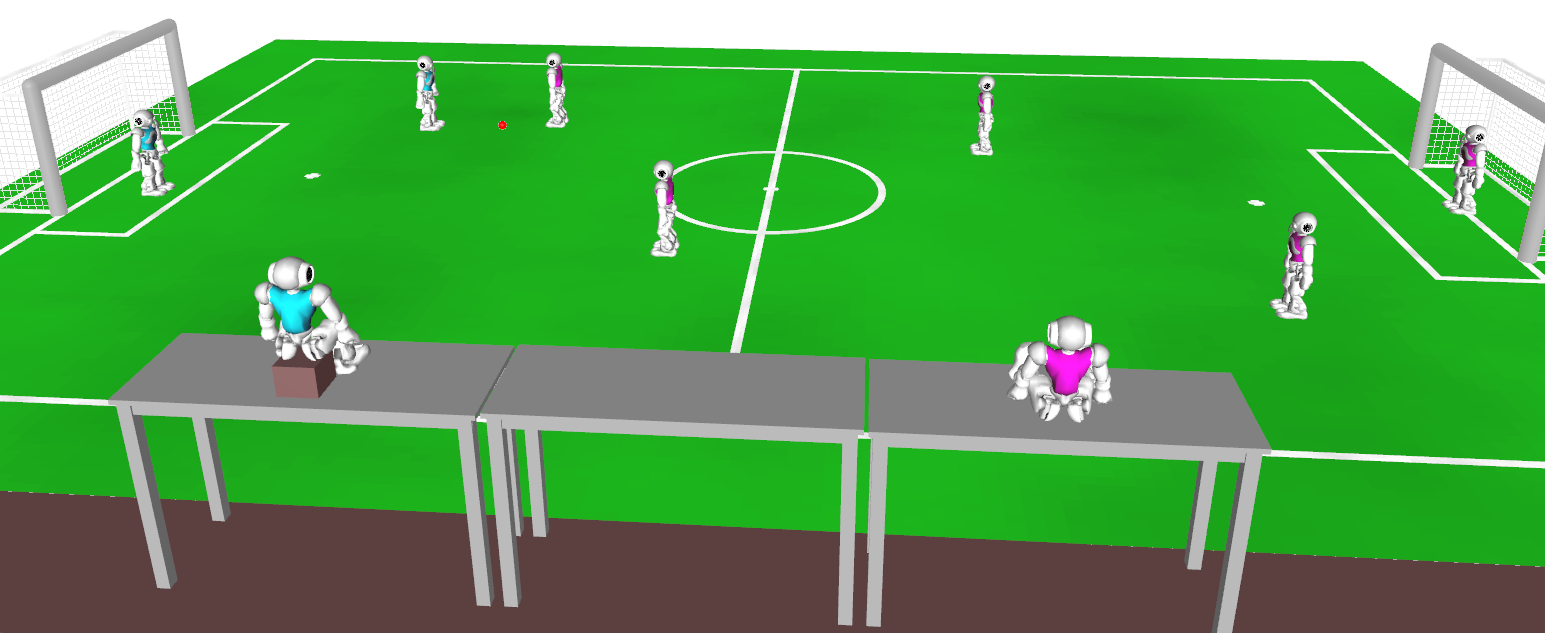
\includegraphics[width=\columnwidth]{figs/coaching-robots}}
  \caption{Two coaching robots observing a game. The left robot is sitting on a seating platform. The right robot sits on the table.}
  \label{fig:coaches}
\end{figure}
 

\subsection{Team Markers}
\label{sec:team_markers}

Robots use colored jersey shirts as team markers. Each jersey shirt has a player number (1-6) printed on it.  The team markers are worn as shown in Figure~\ref{fig:nao_markers}.

\begin{figure}
  \centerline{\begin{tabular}{lll}
      a) & b) & c) \\
      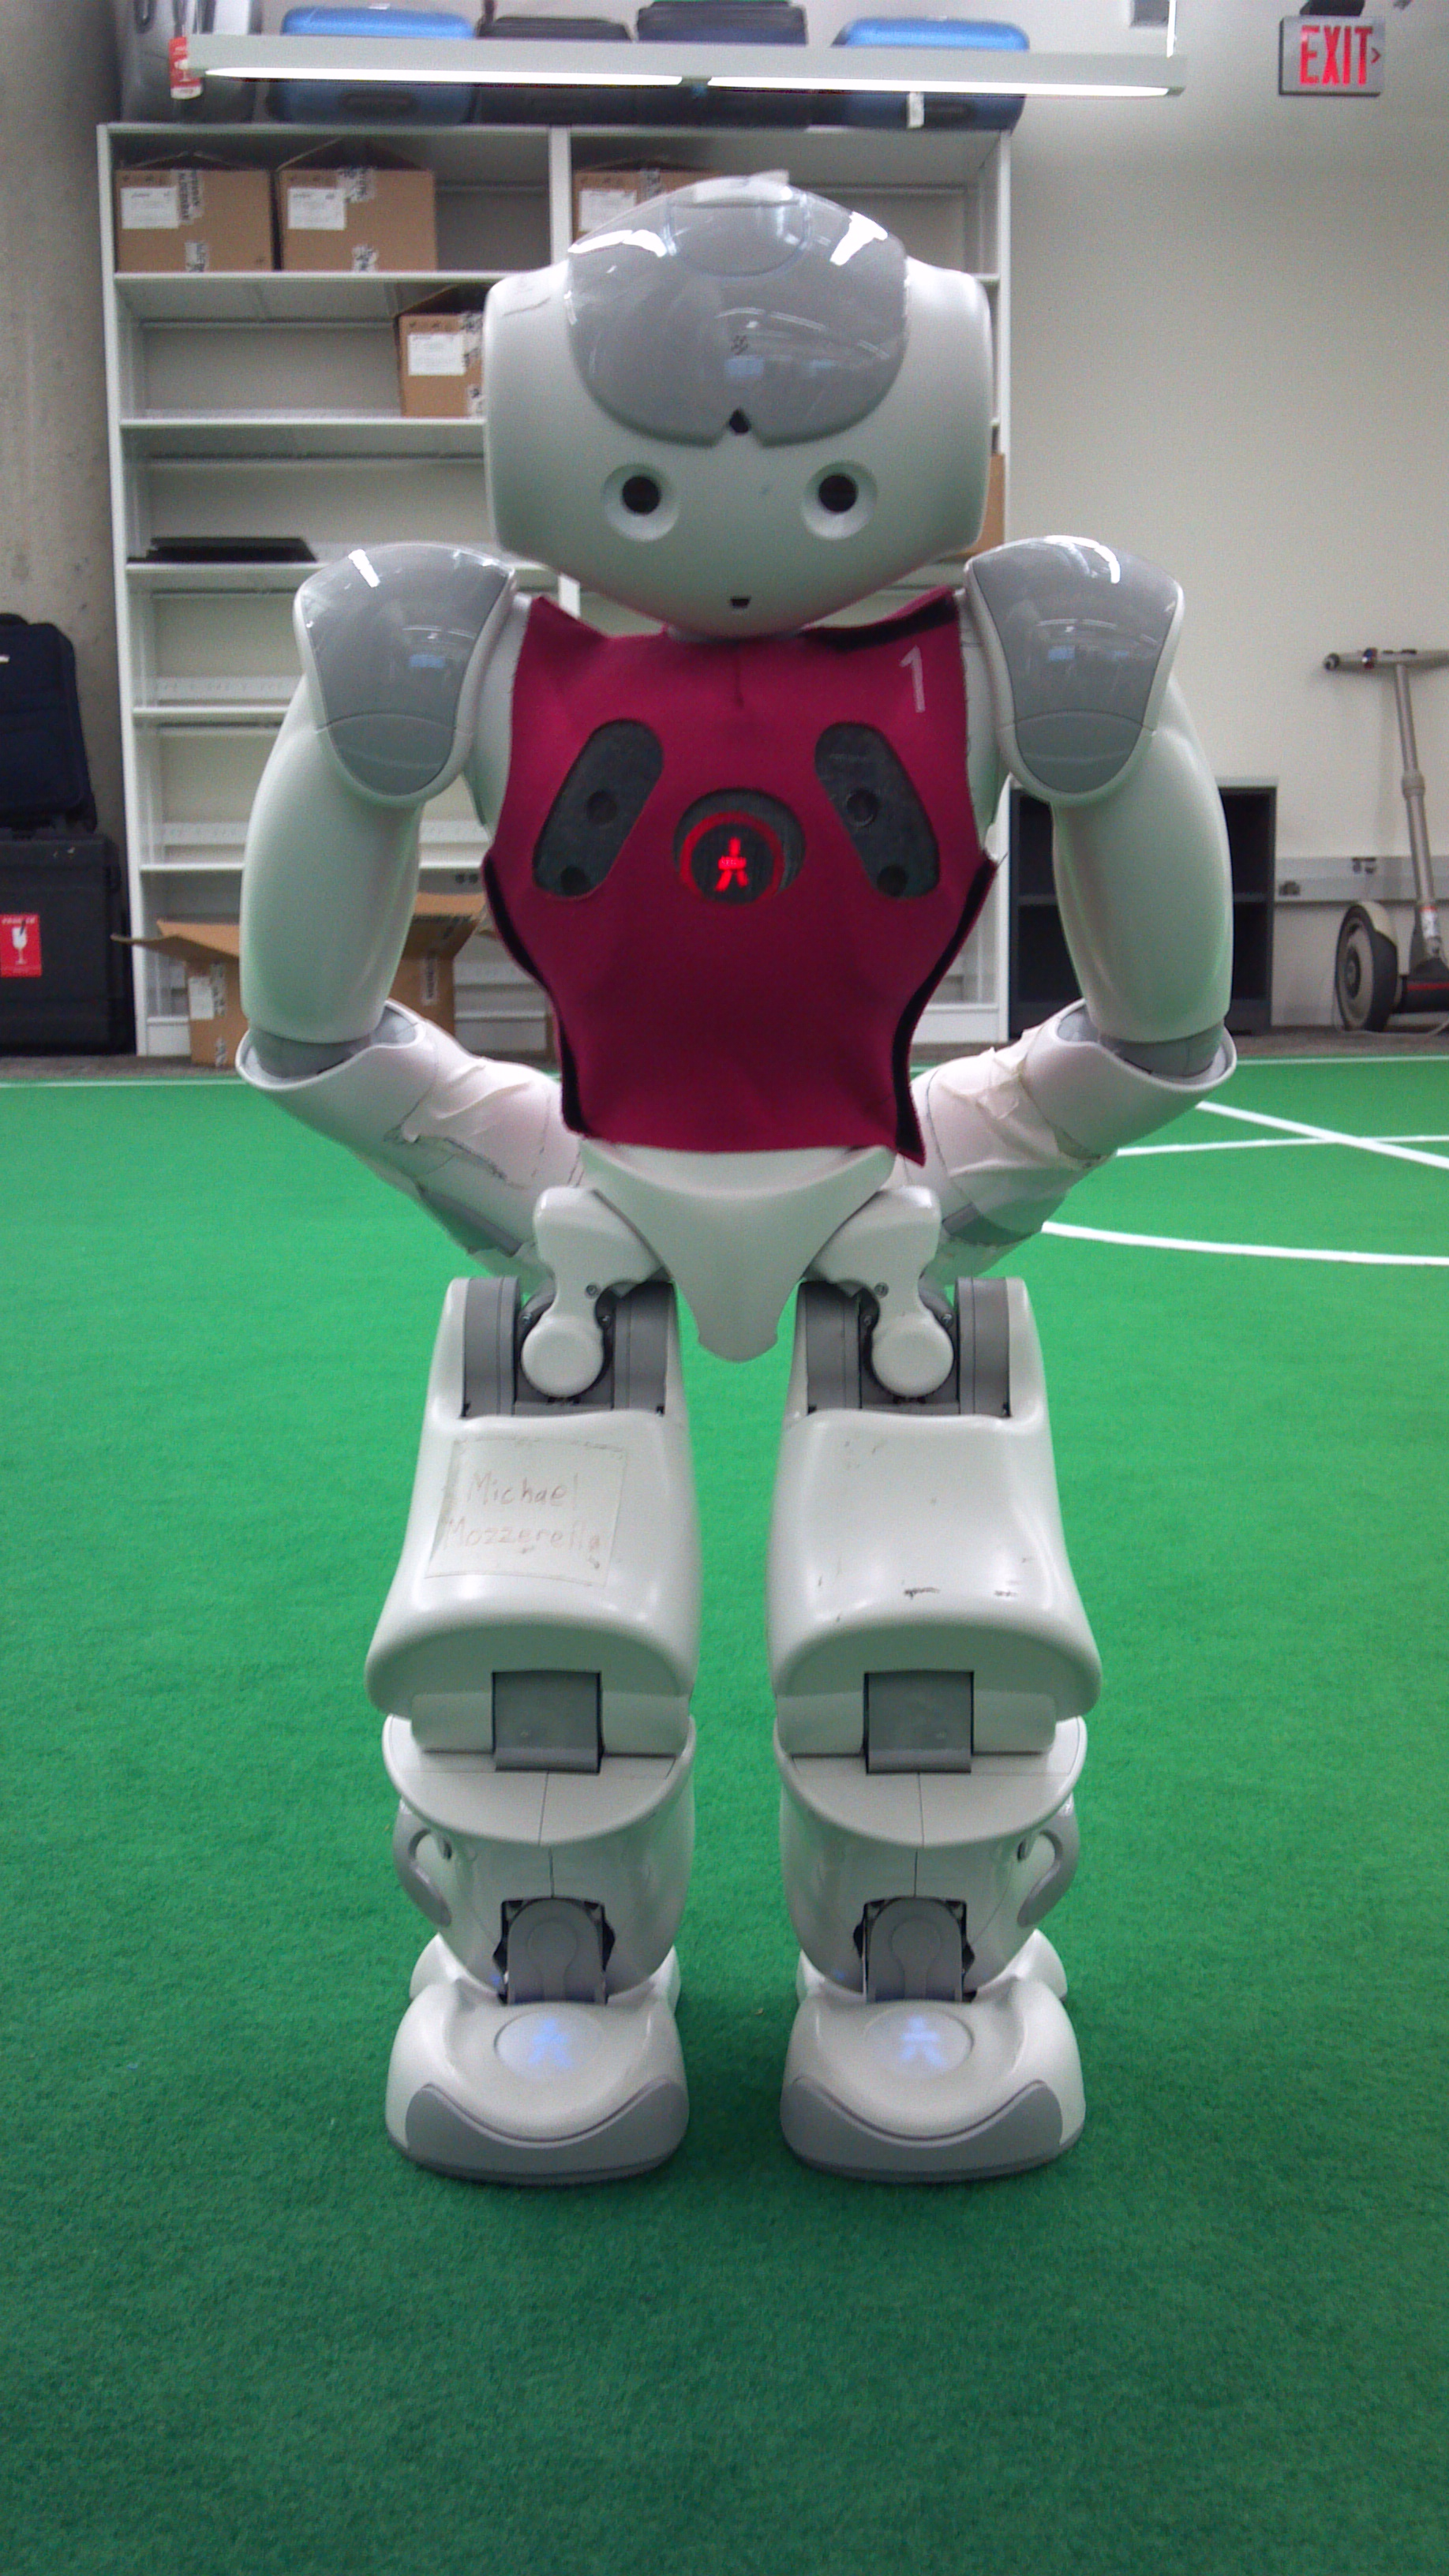
\includegraphics[height=0.28\columnwidth]{figs/front.jpg}&
      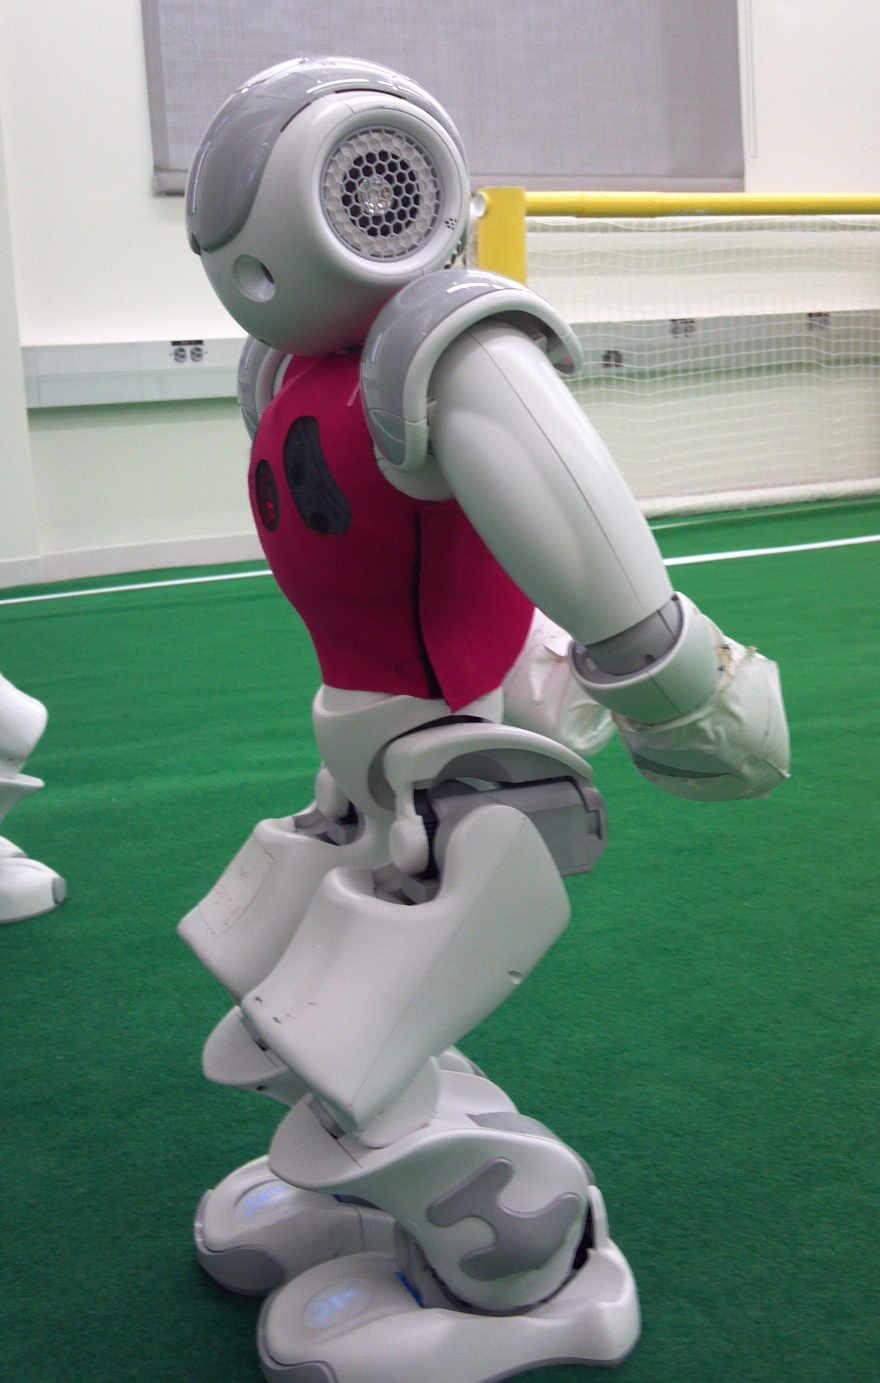
\includegraphics[height=0.28\columnwidth]{figs/side.jpg} &
      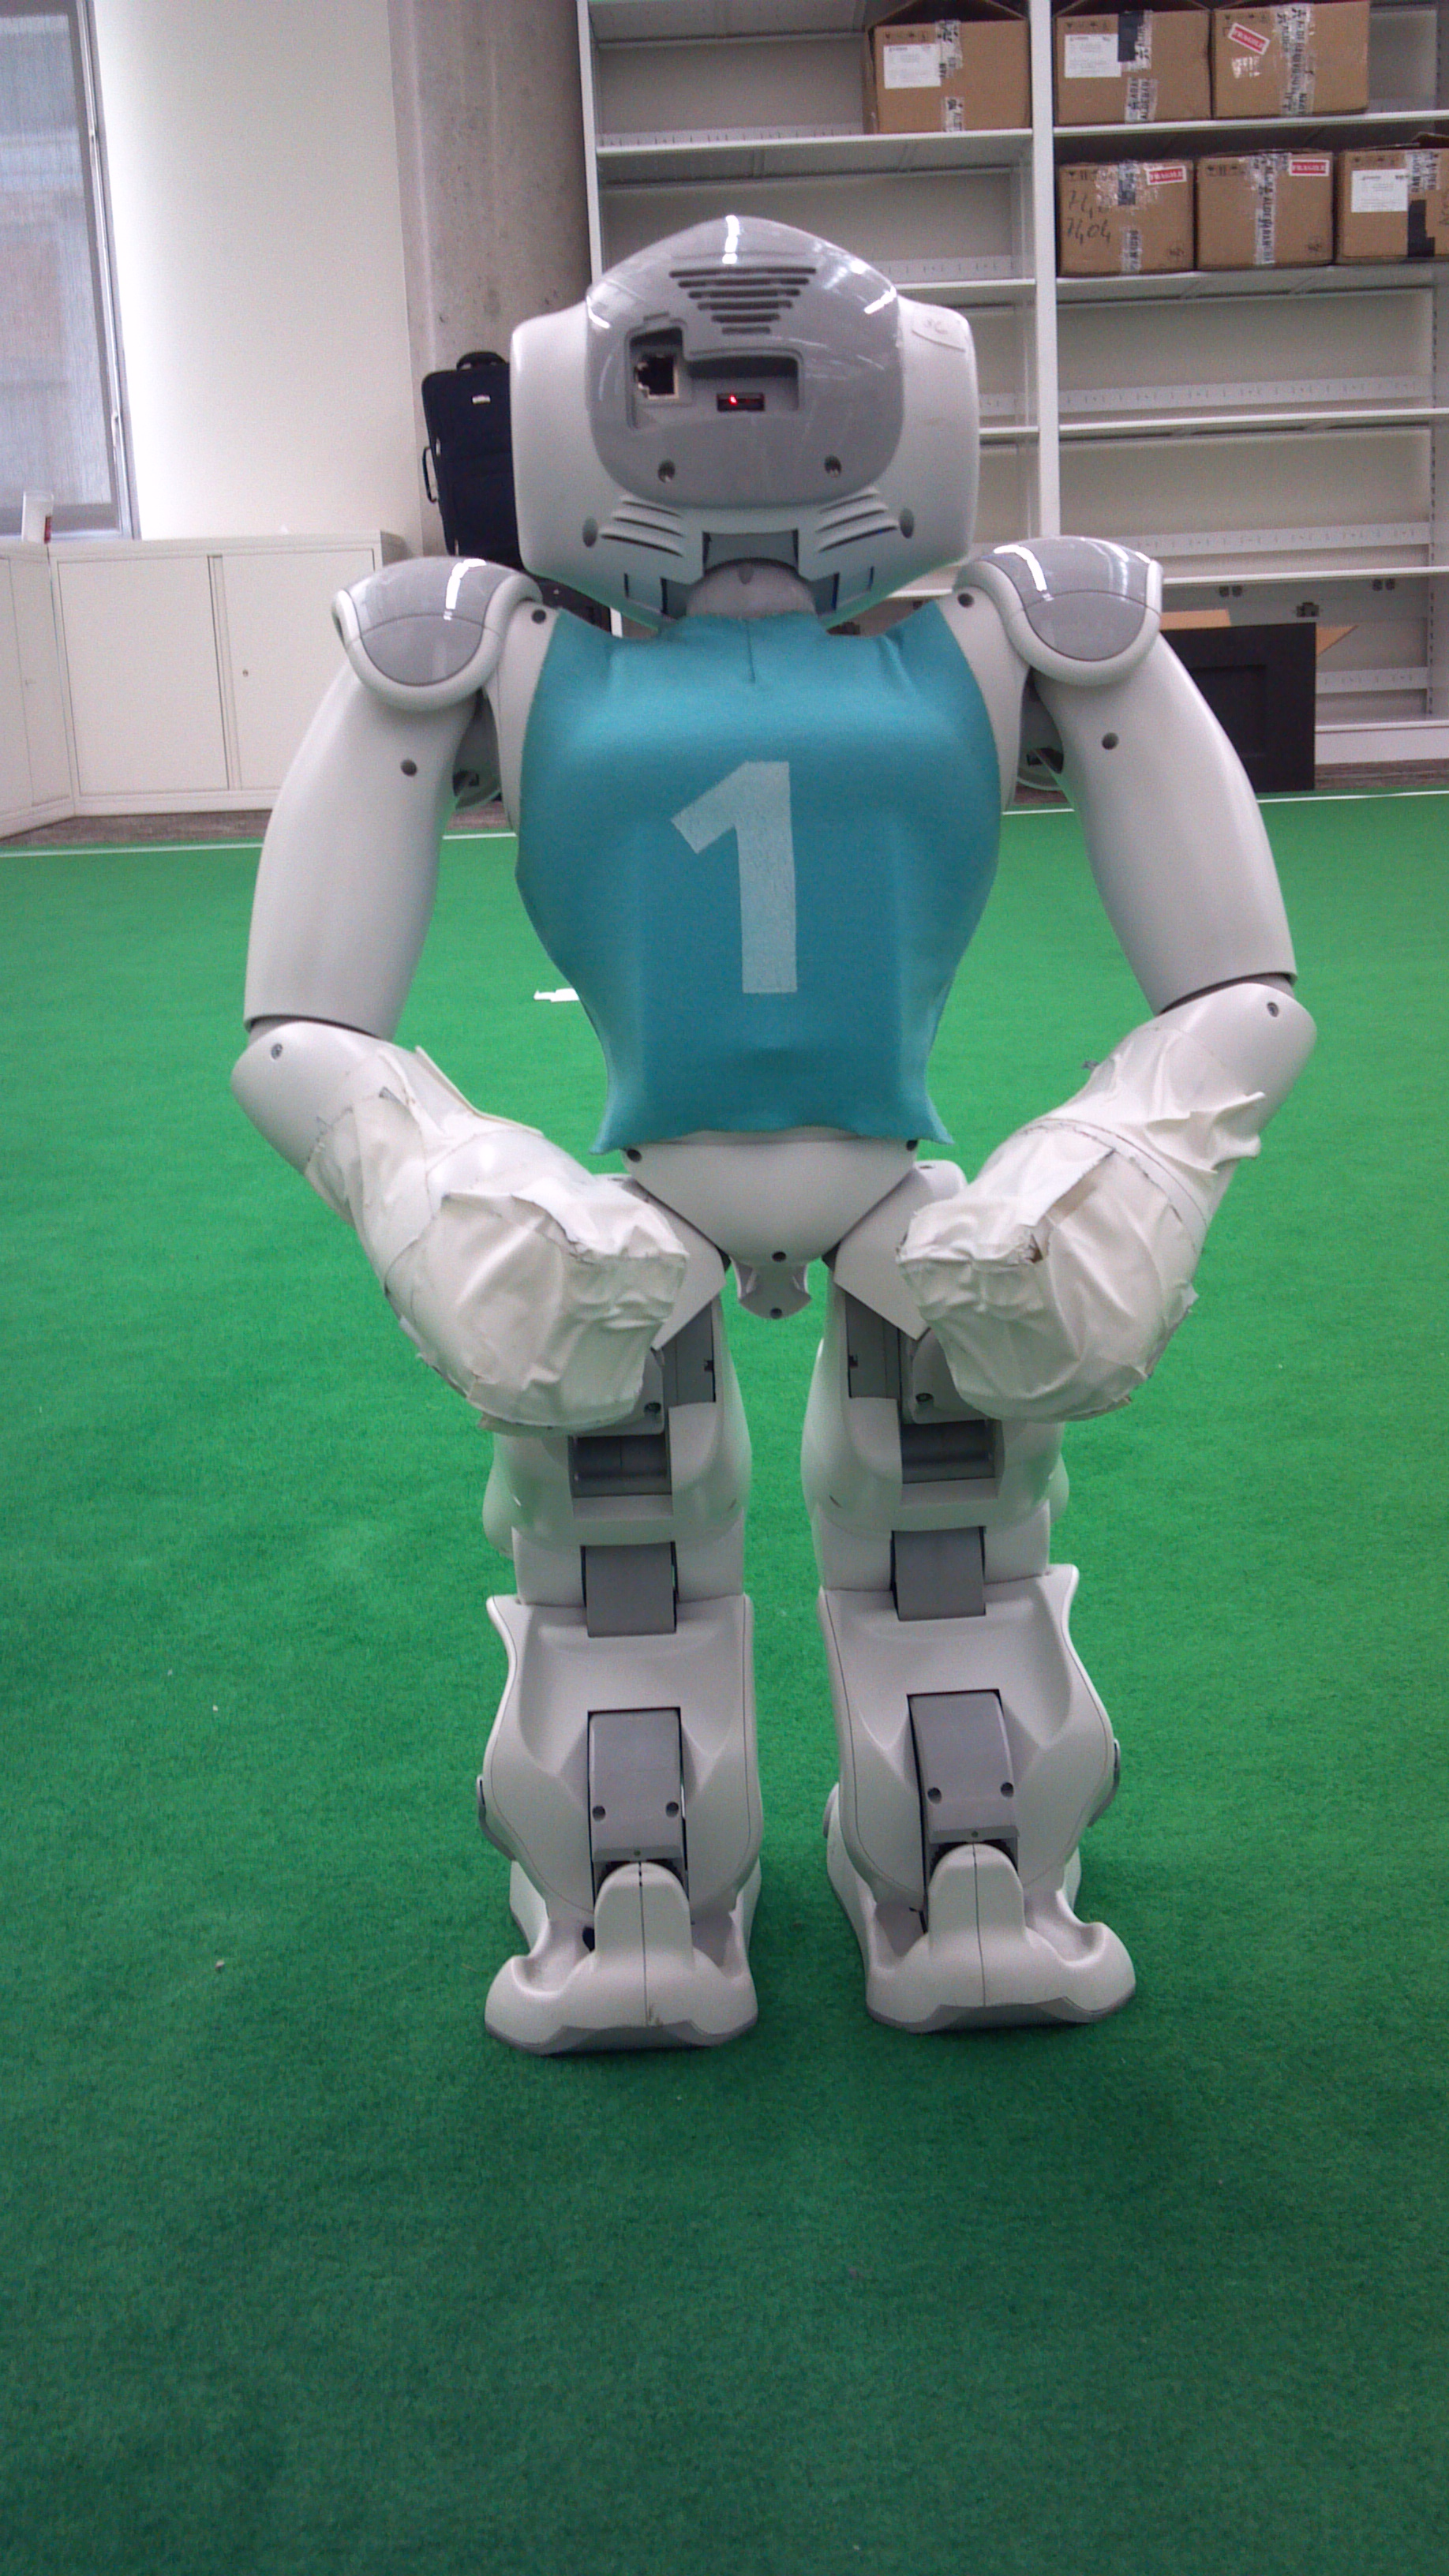
\includegraphics[height=0.28\columnwidth]{figs/back.jpg} 
  \end{tabular} }
  \caption{Team markers. a) Front view. b) Side view. c) Back view.} 
  \label{fig:nao_markers}
\end{figure}


Teams may use jerseys purchased at RoboCup 2013 or RoboCup 2014 (magenta and cyan solid colors) or they may design and manufacture their own jerseys.  Teams opting to design and manufacture their own jerseys may design jerseys in any color (multi and many color jerseys are acceptable), but must follow these guidelines:
\begin{itemize}
\item Jerseys should be the tank top style used at RoboCup 2013/2014 and should cover approximately the same areas of the robot as shown in Figure~\ref{fig:nao_markers}.  The torso LED must be clearly visible.  Jerseys may include the sonar panel used in the 2013/2014 jerseys, although this is not required.
\item Jerseys must have a primary color that comprises at least 70\% of the jersey.
\item Jerseys should not contain distractors, such as large pictures of SPL balls or white stripes on green jerseys.
\item All players on a team must wear identical jerseys, including the goalkeeper.
\item A team must wear the jerseys that it starts a game in for the entire game.
\item Jersey material must be non-reflecting, non-shiny, and non-textured.  Material that is shiny or glittery is also not appropriate.
\item Jerseys should be numbered 1-6 on both sides.  The numbers must be large and {\bf easily} recognized by humans.
\item Teams must have two sets of jerseys that are significantly different in terms of their primary color.
\item Designs must be submitted to \url{rc-spl-tc@lists.robocup.org} for approval by May 1, 2017. If the team has jersey prototypes, they should submit close-up images of a robot wearing the jersey - these images should be taken from front, back, and side angles.  If the team has no prototypes, then designs depicting the expected jersey should be submitted.  All images and designs should be submitted in pdf or jpg format.  If a team does not submit designs by the deadline, they must either use their approved jerseys from RoboCup 2015/2016 or use the magenta and cyan jerseys from RoboCup 2013/2014 (and find a way to obtain these jerseys for themselves).
\end{itemize}

Each team must designate a `home' color and an `away' color when asked about one month before RoboCup.  Teams must wear their `home' jerseys when they are `home' (the first team listed on the schedule).  Teams will wear their `home' jersey when they are `away' (the second team listed on the schedule) as well, unless either the head referee or the GameController program believes the jerseys of two competing teams are too similar.  In this case, the `away' team will then wear their `away' jersey.

Some teams wish to include additional information or logos on their robots.  The following are allowable:
\begin{itemize}
\item Attaching player numbers to the heads and/or legs of the robots.  These numbers should be black with a white background, and should correspond to the number on the robot's jersey.

\item Adding sponsor or team logos to the upper legs of the robots (\cf Figure~\ref{fig:sponsor}). A box drawn around the non-white area of these logos must not cover more that a 25 $\text{cm}^2$ area. At most one logo may be attached per leg --- if you wish to attach more than one logo per leg, email the Technical Committee at least two weeks before the competition.  Depending on the size and design of the logos, this may be allowable.

\item Adding small black and white stickers to the torso of the robots stating the name of the robot, the name of the team, or similar information. These stickers must be small and mostly white.
\end{itemize}

The coaching robot is allowed to wear a custom shirt that has a team-specific design. There are no restrictions regarding colors or patterns. The shirt is allowed to cover the body as well as the upper arms of the coaching robot.

\begin{figure}[b]
  \centerline{\begin{tabular}{ll}
  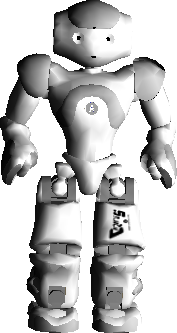
\includegraphics[height=0.35\columnwidth]{figs/naosim_with_logo.png}&
  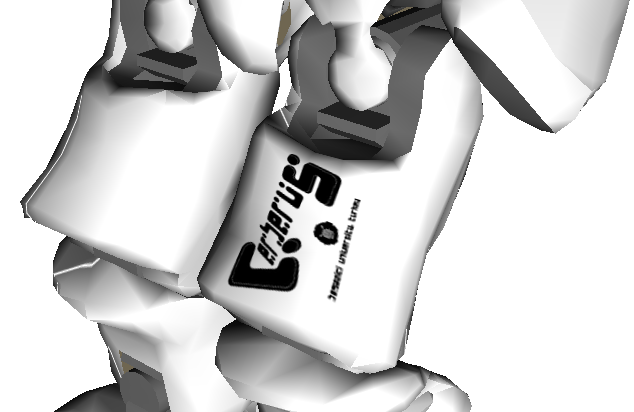
\includegraphics[height=0.35\columnwidth]{figs/naosim_legs_with_logo_closeup.png}
  \end{tabular}}
  \caption{Example Sponsor/Team Logo placement on legs.}
  \label{fig:sponsor}
\end{figure}


\subsection{Communications}

The robots must play without human control. Communication is only allowed among robots on the field and between the robots and the GameController.

\subsubsection{Non-Wireless Communications}
\label{sec:acoustic}
In general there are no restrictions on communication between robots in play on the field using visual signalling (e.g. gestures) or the robot's built-in microphones, speakers, and infrared transceivers. However, communication that causes excessive discomfort to an audience, affects the safety of an audience, or violates normal playing rules is not permitted.

\subsubsection{Wireless Communications}
\label{sec:wireless}
The only wireless hardware allowed to be used by the teams are the wireless network cards built into the NAOs, and the access points provided by the event organizers. All other wireless hardware must be deactivated. A team may be disqualified if one of the team members violates this rule. 

Each team will get a range of IP addresses that can be used both for their robots and their computers. The network configuration (\eg IP addresses, channels, SSIDs, and required encryption) of the fields will be announced at the competition site.

Wireless robot-to-robot communication among the robot players is allowed, as long as it uses the access points provided by the event organizers (using the so-called ad-hoc mode is prohibited), messages are sent via UDP, the SPL standard message packet is used, and not more than five messages per robot per second are sent\footnote{Official status packages that are sent to the GameController can be sent in addition to these five messages.}. The SPL standard message packet is specified in the header \emph{SPLStandardMessage.h} that is distributed with the latest GameController release. Each team will be assigned a range of IP-addresses that can be used for direct robot-to-robot communication. Each team will also be allocated a single UDP port on which broadcast will be permitted.  Specifically, a team's port will be 10000 plus that team's GameController number.

Teams and their robots must not listen into another team's communication.

Robots are not allowed to be connected to access points of fields that are currently running official games of other teams.

The GameController will use UDP to connect to the robots. The source distribution of the GameController provides the header file \emph{RoboCupGameControlData.h} that defines all messages sent by the GameController to the robots. They correspond to the \emph{robot states} described in Section~\ref{sec:robot_states}.

Robots send status updates (defined in \emph{RoboCupGameControlData.h}) to the GameController. These return packets must be addressed directly to the GameController PC (\ie not broadcast) and sent on the GameController return UDP port specified by the symbol \verb!GAMECONTROLLER_RETURN_PORT! in \emph{RoboCupGameControlData.h}.

The coaching robot is not allowed to communicate directly with the robot players, \ie it is neither allowed to send any messages to the players nor is it allowed to listen on ports that are used by players to send messages. Instead, it sends messages to the GameController's coaching interface by using the struct defined in the header \emph{SPLCoachMessage.h} that is distributed with the latest GameController release. These messages have a maximum size of 250 bytes and will be copied by the GameController to its standard messages. However, independent of the sending frequency of a coach, the GameController will accept a new message every second --- all other coach messages will be dropped. There are no limitation on how these messages should be formatted.  Failure to follow these specifications will result in the inability to use the coaching robot until it is able to follow these specifications.

Besides the coaching robot, the use of remote processing/sensing is prohibited.


\newpage


\section{Game Process}
\label{sec:game_process}

\subsection{Structure of the Game}
\label{sec:game_struct}

A game consists of three parts, \ie the first half, a half-time break, and the second half. Each half is 10 minutes counted from the initial kick-off. The half-time break is also ten minutes --- during this time both teams may change robots, change programs, or do anything else that can be done within the time allotted. 

The teams will change the goal defended during the half-time break.

\begin{figure}[t]
\centerline{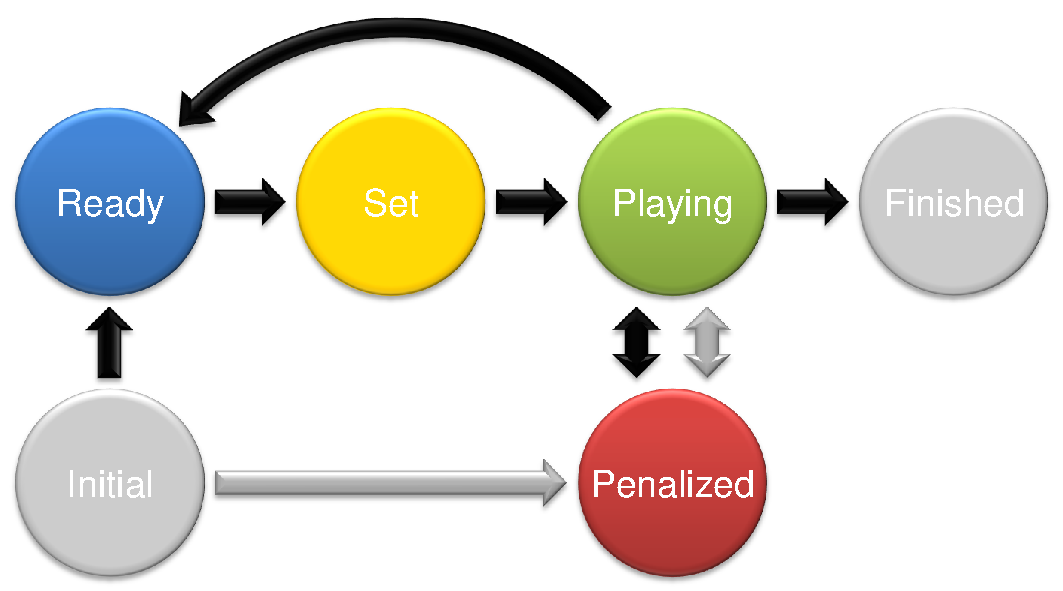
\includegraphics[width=0.9\columnwidth]{figs/states.pdf}}
\caption{Robot states. Button interface transitions are shown in gray. GameController transitions are shown in black. However, any transition possible can actually be sent by the GameController.}
\label{fig:robot_states}
\end{figure}

\subsection{Robot States}
\label{sec:robot_states}

Robots can be in six different states (\cf Figure~\ref{fig:robot_states}). If the wireless is available, these states will be set by the GameController. Teams must implement code to receive and correctly respond to wireless GameController packets, and also give indication of the game state, team color, and the kickoff state.
\emph{If a robot does not respond to either the GameController or the button press interface, then it is not included in the game (technically via a `Request for Pick-up'), and the game starts without the offending robot.}

\begin{description}

\item[Initial.] After booting, the robots are in their \emph{initial} state. The robots are not allowed to be moving in any fashion besides initially standing up. Shortly pressing the chest button will switch the robot to the \emph{penalized} state.

\item[Ready.] In this state, the robots walk to their legal kick-off positions (\cf Section~\ref{sec:kick-off}). They remain in this state, until the head referee decides that there is no significant progress anymore (after a maximum of \KickOffAutoTime). This state is not available if only the button interface is implemented.

Robots may be disentangled by the referees at the start of the Ready state. After that, penalties should be called as normal, but these penalties do not count towards the incremental penalties.  Penalized players should be manually placed during Set (and unpenalized by the GameController).

\item[Set.] In this state, the robots stop and wait for kick-off (\cf Section~\ref{sec:kick-off}). If they are not at legal positions or are fallen and laying in a standing position on the ground, they will be placed manually by the assistant referees to the positions shown in Figure~\ref{fig:ko}. They are allowed to move their heads or get up if fallen before the game (re)starts but they are not otherwise allowed to move their arms or legs or locomote in any fashion. Penalties such as inactive robot, fallen robot, ect may be called as needed. This state is not available if only the button interface is implemented. Robots that do not listen to the GameController will be placed manually. Until the game is (re)started, they are in the \emph{penalized} state.

\item[Playing.] In the \emph{playing} state, the robots are playing soccer. Shortly pressing the chest button will switch the robot to the \emph{penalized} state.

\item[Penalized.] A robot is in this state when it has been penalized. It is not allowed to move in any fashion, \ie also the head has to stop turning. Shortly pressing the chest button will switch the robot back to the \emph{playing} state.

\item[Finished.] This state is reached when a half is finished. This state is not available if only the button interface is implemented.

\end{description}

The GameController Playing signal will be delayed by 15 seconds.  The referee will announce the start of the Playing state with a short whistle blow.  The referee may choose to use any normal sports whistle.  Robots that begin moving their legs or locomoting in any fashion during \emph{set} (\ie before the referee blows the whistle) will be penalized in place on the field via the ``Motion in Set'' (see Section \ref{sec:motion_in_set}) GameController signal (and moved back to their original position if they have moved significantly before becoming penalized) until the GameController transmits the \emph{playing signal}.  Note that responding to a whistle on another field, although unlikely and poor luck, will result in this penalty.

Teams that support the GameController can visualize whether the robot's team has kick-off on the LED of the right foot (off/white) in the states \emph{initial}, \emph{ready} and \emph{set}. The current game state should be displayed on the LED in the torso. The colors corresponding to the game states are:

\begin{itemize}

\item Initial: Off

\item Ready: Blue

\item Set: Yellow

\item Playing: Green

\item Penalized: Red

\item Finished: Off

\end{itemize}

The current GameController requires robots to know both their team number and their robot number within the team. It is each team's responsibility to make sure this is correctly configured. It is recommended that the robot indicates its number within the team on bootup so that this can be easily checked at the start of the game.

\subsection{Goal}
\label{sec:goal}
A goal is achieved when the entire ball (not only the center of the ball) goes over the goal-side edge of the goal line, \ie the ball is completely inside the goal area\footnote{The goal line is part of the field.}. The restart after the goal shall adopt the same rules as the kick-off.

Note that a goal can never be awarded where the last contact of the ball with a robot was by the arm or hand (see Section~\ref{sec:hand_ball}).  The only exception to the rules is a defending goal keeper within its penalty box.

Additionally, a goal can never be awarded when a team scores on themselves and there are no opponent robots on the field that are active (a definition of \emph{active} is given in Sect. \ref{sec:fallenrobots}).  In this case, the goal is not scored and the game will proceed with a throw-in (see Section~\ref{sec:throw_in}).

\subsection{Goal Keeper Save}
\label{sec:goalie_save}
While within its penalty area, a goal keeper may touch the ball with its arms and/or hands.  If a goal keeper is able to lift the ball off of the ground using its arms and/or hands (\ie using at least one arm or hand), and hold it there for at least 1 second, the ball will be moved to one of the two intersections of a throw-in line and the halfway line. Specifically, the ball will be moved to the intersection point closer (regarding the angle) to the goal keeper at the moment of lifting. If the goal keeper is almost aligned with the field's x-axis, the referee should use the intersection point at which a teammate is closer at the moment of lifting.

The robot is not required to lift the ball to a particular height in order for the ball to be considered to be `lifted off of the ground', but lack of contact between the ball and ground must be clearly recognizable by the head referee.

\subsection{Applying Penalties}

See Section~\ref{sec:penalty_procedure}.


\subsection{Initial Kick-off}
\label{sec:initial-kick-off}

The first kick-off at the start of each half is the initial kick-off.
Before the initial kick-off, i.e. before the start of each half, all robots must be in the initial state and must be placed on the sidelines in their own half of the field.
It is up to the team as to which sideline(s) and where exactly on the sidelines the robots are placed.
Once the robots receive the \emph{ready} signal from the GameController, they are to proceed as described in Section~\ref{sec:kick-off}.


\subsection{Kick-off}
\label{sec:kick-off}
For kick-off, the robots listening to the wireless GameController run through three states: \emph{ready}, \emph{set}, and \emph{playing}. Robots not listening to the GameController are simply penalized using the chest button and manually placed for kick-off\footnote{Note that robots being manually placed because they are not listening to the GameController must still be placed in the restricted set of legal positions for manually placed robots. It is to a team's advantage to have their robots listen to the GameController.}.  

In the ready state, the robots should walk to their legal kick-off positions. These positions are always located inside their own side of the field. No player is allowed to touch the halfway line.
The field players of the attacking team can walk to any position within their own half.
The field players of the defending team can walk to any position within their own half, except for inside the center circle.  Only one field player may be within the penalty area during the set state.  If multiple field players are within the penalty area during the set state, the robot(s) closer to center field should be placed manually by the assistant referees to the closest position(s) (as shown in Figure~\ref{fig:ko}) in which a team mate is not already positioned within 1 meter.

If robots incur penalties during Ready state, the penalty is manual placement by the assistant referees. Note that these penalties do not follow the standard removal procedure, and hence do not count towards the incremental penalty count.

The robots have a maximum of \KickOffAutoTime to reach their positions. If all the robots have reached legal positions and have stopped, or if \KickOffAutoTime have passed, the robots will be switched into the \emph{set} state, in which they must stop walking. Each robot that is not at a legal position at this point in time will be placed by the assistant referees in the closest manual position (see Figure~\ref{fig:ko}) that does not already have a team mate within 1 meter.
Robots that are legally positioned will not be moved by the assistant referees unless a manual position is requested by the team leader.
\emph{In the case where the team leader requests manual placement, all robots on that team --- including those penalized in place for ``Motion in Set'' --- are manually positioned.}  However, the penalty persists for those players penalized for ``Motion in Set''.


\begin{figure}[t]
\centerline{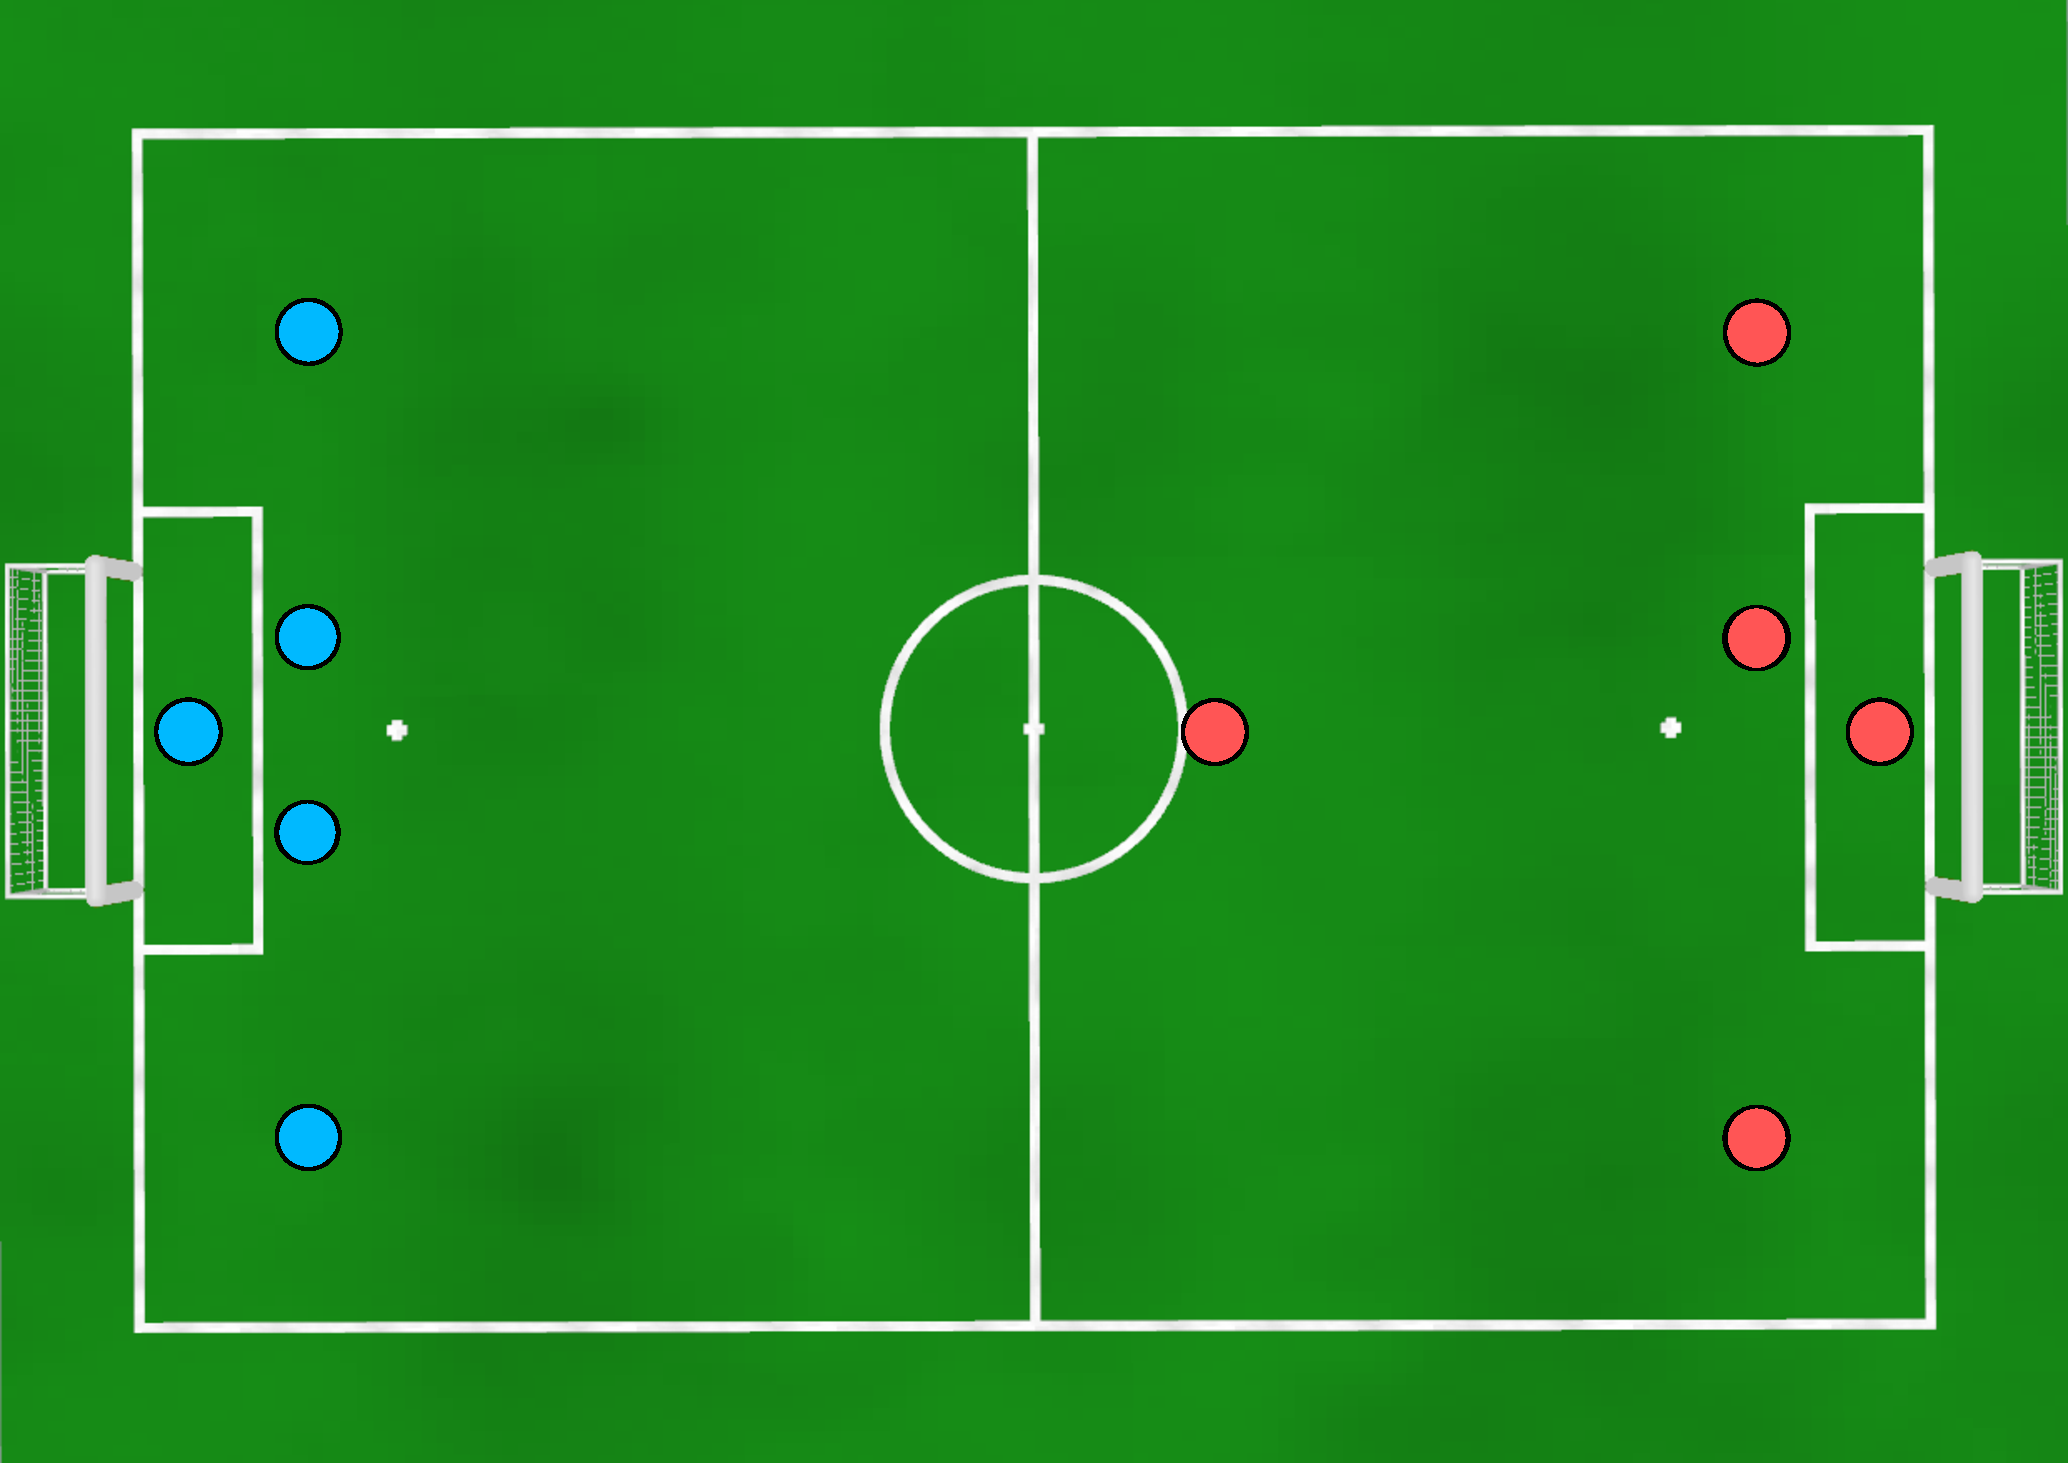
\includegraphics[width=\columnwidth]{figs/manual-placement-2015.pdf}}
\caption{Manual setup for kick-off.  The attacking team is on the right.}
\label{fig:ko}
\end{figure}

The legal positions for manually positioned robots are shown in Figure~\ref{fig:ko}. The kicking-off robot is placed such that its feet touch the center circle (but are not inside it), right in front of the penalty mark. The goal keepers for each team are placed at the center of the penalty box, with their feet immediately in front of the end-line.

To assist the assistant referees in placing the robots manually when needed or requested, small Xs will be marked on the field using a black felt-tip pen in the spots where manually placed robots should go.  These marks should be small, such that they are visible to humans but invisible to robots.

As autonomously placed robots are allowed to be much closer to the ball, successful autonomous placement results in a significant advantage over manual placement.

Just after the \emph{set} state is called, the ball is placed on the center point of the center circle by one of the referees. If it is moved by one of the robots during Set it is replaced by one of the referees.

After the head referee has signaled the kick-off, the robot's state is switched to \emph{playing} (again either by the GameController or manually), in which they can actually play soccer.
The defensive team must stay outside of the center circle until the ball is in play.  The ball is in play once it is touched by the attacking team or once \emph{10 seconds} have elapsed in the playing state. If a defensive player enters the center circle before the ball is in play, the ``Illegal Defender'' penalty is applied (\cf Section~\ref{sec:illegal_defender}).

Note that in some cases a goal can not be scored from within the center circle on kick-off. See Section~\ref{sec:kick-off_shot} for details.

\subsection{Throw-in}
\label{sec:throw_in}

A ball is considered to have left the field when there is no part of the ball over the outside of the boundary line (\ie the line itself is in). If the ball leaves the field it will be replaced on the field by an assistant referee. There is \emph{no} stoppage in play.

Throw-in lines will be marked (as dots at the end of the throw-in lines and short dashes along the line) by the technical committee at the start of competition with a felt-tip pen --- these lines are intended to stay invisible to robots but provide a guide to referees.  These two throw-in lines are 400 mm away from the sidelines and run parallel to them inside the playing area.  Each throw-in line is 7m long.

If the ball goes over a sideline then the assistant referee will replace the ball back on the field on the throw-in line on the same side of the field as the ball went out of play.

The ball will be replaced on the throw-in line at the farthest back of these two locations: a) one meter back from the point it went out or b) one meter back from the location of the kicking robot. We define `back' as being towards the goal of the team that last touched the ball. Note that if the one meter placement would cause the ball to be placed off the end of the throw-in line, then it should be placed at the end of the throw-in line, and not beyond.

If the ball goes over an end-line then the assistant referee will replace the ball back on the field according to the following rules:

\begin{itemize}

\item If the ball was last touched by the defensive team then the ball is replaced on the closest endpoint of the throw-in line.

\item If the ball was touched by the offensive team, the ball is replaced on
the throw-in line at the farthest back of these two locations: a) one
meter back from the location of the kicking robot, or b) at the halfway
line.

\end{itemize}

Balls are deemed to be out based on the team that last touched the ball, irrespective of who actually kicked the ball.  In these examples, ``red half of the field'' refers to the half the red team is defending.

\paragraph{Example 1.} The red goal keeper kicks the ball out the end of the field to the right of the goal. The ball is placed on the endpoint of the throw-in line to the right of the goal.

\paragraph{Example 2.} A blue robot on the red half of the field kicks the ball out the end of the field to the right of the goal the red team is defending. The ball is placed on the intersection of the right throw-in line and the halfway line.

\paragraph{Example 3.} A blue robot on the blue half of the field kicks the ball out the end of the field to the right of the goal the red team is defending. The ball is placed on one meter behind the robot on the right throw-in line.

\paragraph{Example 4.} A blue robot at midfield kicks the ball over the left sideline 2 meters into the red half of the field. The ball is replaced on the left throw-in line 1 meter into the blue half of the field (one meter behind the robot).

\paragraph{Example 5.} A blue robot at midfield kicks the ball over the left sideline 2 meters into the blue half of the field (towards its own goal). The ball is replaced on the left throw-in line 3 meters into the blue half of the field.

\paragraph{Example 6.} A blue robot kicks the ball but the ball touches a red robot at midfield before leaving the field near the center line. The ball is regarded as out by red and therefore is replaced on the throw-in line 1 meter closer to the goal the red team is defending.


\subsection{Game Stuck}
\label{sec:game_stuck}

In the event of no substantial change in the game state for 30 seconds, this is considered a game stuck.  ``Substantial change'' can consist of a robot seeing and moving towards the ball OR robots exploring the field (presumably in an attempt to find the ball).

The main referee has two options how to solve the game stuck and to reestablish the chance of progress in the game. The intention of the game stuck rule is to achieve progress with as little intervention as possible, \ie the \emph{Local Game Stuck} rule will be preferred, but only if there is a chance that its application will result in progress in the game.

\subsubsection{Local Game Stuck}
\label{sec:game_stuck:local}

If one robot is preventing the game from proceeding --- perhaps by circling the ball repeatedly without kicking the ball --- it is recommended to improve progress by removing this one robot.

When Local Game Stuck is called, the nearest robot to the ball will be penalized and removed for 45 seconds (Section \ref{sec:pen_local_game_stuck}). Local Game Stuck penalties do not following the standard removal procedure, and hence do not count towards the incremental penalty count.

\subsubsection{Global Game Stuck}
\label{sec:game_stuck:global}

If no robots have made progress towards the ball or began to explore the field in 30 seconds, Global Game Stuck should be called be called on the team whose robot is not nearest the ball.

Once the referee calls Global Game Stuck, players enter the Ready state, and a new kick-off is awarded to the team that was closer to the ball when the Global Game Stuck was called. A global game stuck can only be called if at least one robot has touched the ball since the previous kick-off.

\subsection{Request for Pick-up}
\label{sec:request_for_pickup}

Either team may request that one of their players be picked up (called ``Request for Pick-up'').  Players in the Playing state may only be picked up for hardware failures.  Players in all other states may be picked up for any reason.

Basically every change (hardware or software) is allowed during a request for pick-up. In particular,
it is permitted to change batteries, fix mechanical problems, reboot the robots, and change configuration files.
It is discouraged to change the robot's control program, \textbf{but not forbidden}.
It is also allowed to replace a broken robot by a substitute robot.

Any strategic ``Request for Pick-up'' is not allowed, i.e. gaining an advantage by removing the robot from the game.
In this case, the head referee will indicate when the robot is no longer affecting play and can be removed from the field by an assistant referee.

To prevent mistakes and confusion during games, only team leaders should make a ``Request for Pick-up'', and only one designated person per team shall accept the robot from the referee, and hand it back after fixing the problem.
The returning robot may be returned following the normal replacement procedure at any point within Ready or Set states.  In Playing, the robot may return once at least 45 seconds have elapsed since the robot was removed from play. Note that this penalty does not follow the standard removal procedure, and hence do not count towards the incremental penalty count.

The robot should be returned to the assistant referees in the \emph{penalized} state.

\subsection{Request for Timeout}
\label{sec:request_for_timeout}

At any stoppage of play (after a goal, stuck game, before a half, etc.) either team may call a timeout. Each team can call a \textbf{maximum of 1 timeout per game} with a total time totaling no more than \textbf{5 minutes}. During this time, both teams may change robots, change programs, or anything else that can be done within the time allotted.  It is allowable to call one timeout before a penalty shootout or between penalty kicks if the penalty shootout directly follows a game in which the team did not use a timeout.

The timeout ends when the team that called the timeout says they are finished, at which time they must be ready to play. The other team must be ready to play at the time the timeout runs out, or \textbf{2 minutes} after a prematurely called end of the timeout, whichever is earlier. If the other team is not ready to play in time, it has to call a timeout of its own.
  
The clock stops during timeouts, even during the preliminaries.

After the completion of the timeout, the game resumes with a kick off for the team which did not call the timeout.

If a team is not ready to play at the assigned time for a game, the referee will call the timeout for that team. After the expiration of such a timeout, if the team is still not ready to play then the referee shall start the game with only one team on the field.  The team that was not ready can return its robots to the field as per the rules for ``Request for Pick-up''. If both teams are not ready, the referee will call timeouts for both teams. This ``double timeout'' expires after 10 minutes.

\subsection{Referee Timeout}
\label{sec:referee_timeout}
The head official may call a timeout at any stoppage of play if he or she deems it necessary.  A referee timeout should only be called in dire circumstances --- one example might be when the power to the wireless router is down.  However, when and whether to call a referee timeout is left up to the head referee.

Referees may call multiple timeouts during a game if needed.  Teams may do anything during these timeouts, but they must be ready to play \textbf{2 minutes} after the referee ends a timeout.  The referee should end the timeout once he or she believes the circumstance for which the timeout was called has been resolved.  In cases where the circumstance for which the timeout was called is not resolved within 10 minutes, the chair of the technical committee should be consulted regarding when/if play should continue.

The team who would have kicked off if the timeout had not been called shall kickoff when the game resumes.

\subsection{Extra Time}
\label{sec:extra_time}
The head official may decide to add time to the clock if a substantial delay (such as an enormous wireless delay) causes excessive game time to be lost.  The decision to add time to the clock should be made immediately after the incident.  The person working the GameController should execute this addition of time using the GameController interface.

\subsection{Mercy Rule}
\label{sec:mercy_rule}
A game will conclude once the game score shows a goal difference of 10.  Ending the game is mandatory once a goal difference of 10 is reached.

\subsection{Rules for Forfeiting}
\label{sec:forfeit}

Teams who do not make a good faith effort to participate in a scheduled game are considered to forfeit the game.  In the case of a forfeit, a note will be added to the Penalty Counts list kept by the league, which may affect qualification in future years.

If a team notifies the technical committee that they wish to forfeit less than two hours before their scheduled game time, simply fails to show up for their game, or decides during their game that they wish to forfeit, then the opposing team will play the match against an empty field.  However, any own goals will not be scored.  Hence, after an opponent forfeits, the team playing against an empty field cannot do worse than they were doing at the time the opponent decided to forfeit.  Teams may choose to forfeit at any stoppage of play.  However, once a forfeit is announced, they may not reverse this decision.

If a team notifies the technical committee that they wish to forfeit at least two hours before their schedule game time, the following procedure will be followed.

\begin{itemize}
\item If a team chooses to forfeit a match in the round robin games the other team plays the match against an empty field.  However, any own goals will not be scored.
\item If a team chooses to forfeit in a knock-out game which it reached directly after a round robin group, it will be replaced by its runner up in that round robin group.
\item If a team chooses to forfeit in a knock-out game which it reached after a previous knock-out game (e.g. semi final after winning the quarter final), it will be replaced by the team that it eliminated in the previous round.
\item If a team chooses to forfeit the final and the final is scheduled to occur after the 3rd place game, it will be replaced by the 3rd place winner, and the 4th place team will become 3rd place. No new 4th place will be selected.
\item If a team chooses to forfeit the final and the 3rd place game is scheduled to occur after the final, it will be replaced by the team that lost to the forfeiting team in the previous semifinals. No 3rd place game will be played.
\end{itemize}

Note that there are a few unlikely cases that are not covered by these rules.  If a situation is not covered by these rules, the technical committee and the organizing committee will work together to make a decision.

\subsection{Penalty Kick Shoot-out}
\label{sec:penalty_shoot-out}

A penalty kick shoot-out is used to determine the outcome of a tied game when an outcome is required (for example, when team progression is tied on all tie-break factors, during the intermediate round, quarter finals, semi finals, third place or final). 
There will be a five minute break between the end of the game and the start of the penalty kicks.
At all stages of the competition, the penalty kick shoot-out will consist of three penalty shots per team.
All penalty shots are taken against the same goal\footnote{Which goal to take for the shoot-out is decided in accordance with the teams, or otherwise by a coin toss.}. At the conclusion of these shots the team that has scored the most goals will be declared the winner. Note that a winner can be declared before the conclusion of the penalty shoot-out if a team can no longer win, for example, a team requires 2 goals to win but only has 1 attempt remaining. If the two teams still remain tied then a sudden death shoot-out will follow until a definite winner is found.

Teams are allowed to switch to specially designed software for a penalty kick.  Moreover, teams are allowed to replace their robot after each penalty shot attempt if desired.  However, all robots (including the replacements) must be ready and handed over to the referees before the penalty shootout begins. After the start of the penalty shootout, no additional code changes are allowed. No timeouts may be called during the penalty shootout.

The procedure for each of the first 3 attempts is described in Section~\ref{sec:penalty_kick}. If after three penalty kicks by each team there is no result (that is, each team has scored the same number of goals), then the decision will be made by the following sudden death shoot-out procedure in \ref{sec:sudden_death_shoot_out}.

\subsubsection{Penalty Kick}
\label{sec:penalty_kick}

A penalty kick is carried out with one attacking robot and one opposing goal keeper. Robots that will not participate in the shootout (including the coach) must not be on the wifi network and must stay outside of the field. Replacement robots that might participate and have been handed to referees must not be transmitting on the wifi network until or unless it is their turn to play.

The first (left) team in the GameController will perform the first penalty kick.

Referees place the attacking robot, the goal keeper robot, and the ball. The ball is placed on the penalty spot, at the end of the field closest to the goal being defended. The attacking robot is positioned 1 meter behind the penalty spot, facing the ball.  This spot is denoted with a small dot made with a felt-tip pen. The goal keeper is placed with its feet on the goal line and in the center of the goal.

Neither robot shall move their legs before the penalty kick starts. Movements of the robot's head and arms are allowed as long as the robot does not locomote. Technically, the robots are in the \emph{set} state when waiting for the penalty kick to start. If robots are not listening to the GameController, they are in the \emph{penalized} state instead. The robots are started by switching to the \emph{playing} state.

The attacking robot is only allowed to contact the ball once.  The time limit for the kicker is 45 seconds after the penalty kick starts. The ball must be in the goal within this time limit in order to count as a goal.

A penalty shot is over when the ball has come to a full stop after the first contact by the attacking robot, either in favor of the attacker if a goal has been scored, or in favor of the defending team if the goal keeper successfully blocked or if the ball just did not reach the goal line.

The goal keeper is not allowed to touch a ball that is completely outside the penalty area, where the line is part of the penalty area. If the goal keeper touches the ball when the ball is completely outside the penalty area, then a goal will be awarded to the attacking team.

All the rules such as ``Ball Holding'', ``Pushing'' and others are also applied during the penalty kick.  A goal keeper will not be penalized for inactivity during a penalty kick, provided its stiffness is on. Other penalties are applied as usual.

The attacking robot will be indicated by the GameController using the kick-off flag, \ie the kick-off team is the attacking one.

\subsubsection{Sudden Death Shoot-Out}
\label{sec:sudden_death_shoot_out}

The time limit for sudden death penalty shots is 45 seconds.

These attempts will be timed (that is, for a goal scored, how long did it take to score the goal) and measured if a goal is not scored (that is, what is the shortest distance between the final ball position and the goal line segment between the goal posts) by the referee. After these attempts, the game decision will be made as follows:

\begin{enumerate}

\item If only one team scores a goal, that team wins.

\item If both teams score a goal, then if one team is timed to have scored at least 2 seconds faster than the other team, the faster team wins. Otherwise, the sudden death shoot-out is repeated.

\item If neither team scores a goal, then if one team is measured to have moved the ball more than 50~mm closer to the goal than the other team, the closer team wins. Otherwise, the sudden death shoot-out is repeated.

\item If neither team has touched the ball during the shoot-out, the referee will toss a coin to decide the game.

\end{enumerate}


\newpage


\section{Forbidden Actions and Penalties}
\label{sec:forbidden_act}

The following actions are forbidden. In general, when a penalty applies, the robot shall be replaced, not the ball. For penalties that are timed, the penalty time is considered to be over whenever the game time stops (for goals, half-time, and game stuck).

\subsection{Locomotion Type}
\label{sec:locomotion_type}

Robots should clearly demonstrate bipedal walking similar to human walking. Other types of locomotion involving other parts than feet (crawling etc.) are strictly forbidden. It is duty of the head referee to decide whether a robot's locomotion is appropriate. Robots using inappropriate locomotion types will be removed via `Request for Pick-up' until they are able to show appropriate locomotion.

\subsection{Motion in Set}
\label{sec:motion_in_set}

Robots may not exit the Set state until either the referee's whistle is detected or a GameController Playing signal has been received.  Players that leave the Set state prematurely will be called for ``Motion in Set'' and penalized in place on the field.  They will then be unable to move until they receive the GameController Playing signal.  Motion in Set penalties do not following the standard removal procedure, and hence do not count towards the incremental penalty count.

\subsubsection{Local Game Stuck}
\label{sec:pen_local_game_stuck}

A robot should not prevent the game from proceeding.  In some cases, the head referee may decide to remove a player if doing so is likely to help the game proceed (see Section \ref{sec:game_stuck:local}).

When Local Game Stuck is called, the nearest robot to the ball will be penalized and removed for 45 seconds. Local Game Stuck penalties do not following the standard removal procedure, and hence do not count towards the incremental penalty count.

\subsection{Penalty Procedure}
\label{sec:penalty_procedure}

When a robot commits a foul, the head referee shall call out the infraction committed, the primary jersey color of the robot, and the jersey number of the robot. The penalty for the infraction will be applied immediately by an assistant referee. The assistant referees should perform the actual movement of the robots for the penalty so that the head referee can continue focusing on the game. The operator of the GameController will send the appropriate signal to the robots indicating the infraction committed.

\subsection{Standard Removal Penalty}
\label{sec:removal_penalty}

Unless otherwise stated, all infractions in this league result in the removal of the infringing robot from the field of play for a particular amount of time, after which it will be returned to the field of play. This process is called the standard removal penalty, and a detailed description of the process follows.

When the head referee indicates a foul has been committed that results in the standard removal penalty, the assistant referee closest to the robot will remove the robot immediately from the field of play. The robot should be removed in such a way as to minimize the movement of the other robots and the ball. If the ball is inadvertently moved when removing the robot, the ball should be replaced to the position it was in when the robot was removed.

The operator of the GameController will send the appropriate signal to the robot indicating the infraction committed. If the wireless is not working and the penalty is timed, the assistant referee handling the robot will reset the robot into the \emph{penalized} state for the duration of the penalty. After a penalty is signaled to the robot, it is not allowed to move in any fashion, such as being in the \emph{initial} state. The removed robot will be placed outside of the field facing away from the field of play.

Unless otherwise specified, penalty times become incrementally longer each time a team commits any infraction.  Specifically, the first infraction will result in a penalty time of 45 seconds, the second infraction (of any type) will result in a penalty time of 50 seconds, the third infraction (of any type) will result in a penalty time of 55 seconds, ect.  The counter for each team's infractions will reset at half-time.  

The GameController will keep track of the time of the penalty. The operator of the GameController will signal the assistant referees when the penalty is 10 seconds from being over, so that one of them can place the robot in the half of the field which this robot's team is defending on the sideline that is farther from the ball. The robot should be placed close to the position where the penalty point projects on the sideline. This is illustrated in Figure~\ref{fig:penalty_re-entry_points}. 

If there is another robot already in this position, the robot should be replaced at a nearby location along the sideline. When finding a nearby location, locations away from the ball should be preferred, but they \textbf{must} still be in the robot's own half, so that the symmetry of the field can be resolved by the robot's localization system.

With approximately 5 seconds left before the penalty ends, the robot should be turned to face towards the opposite sideline.

\begin{figure}[t]
\centerline{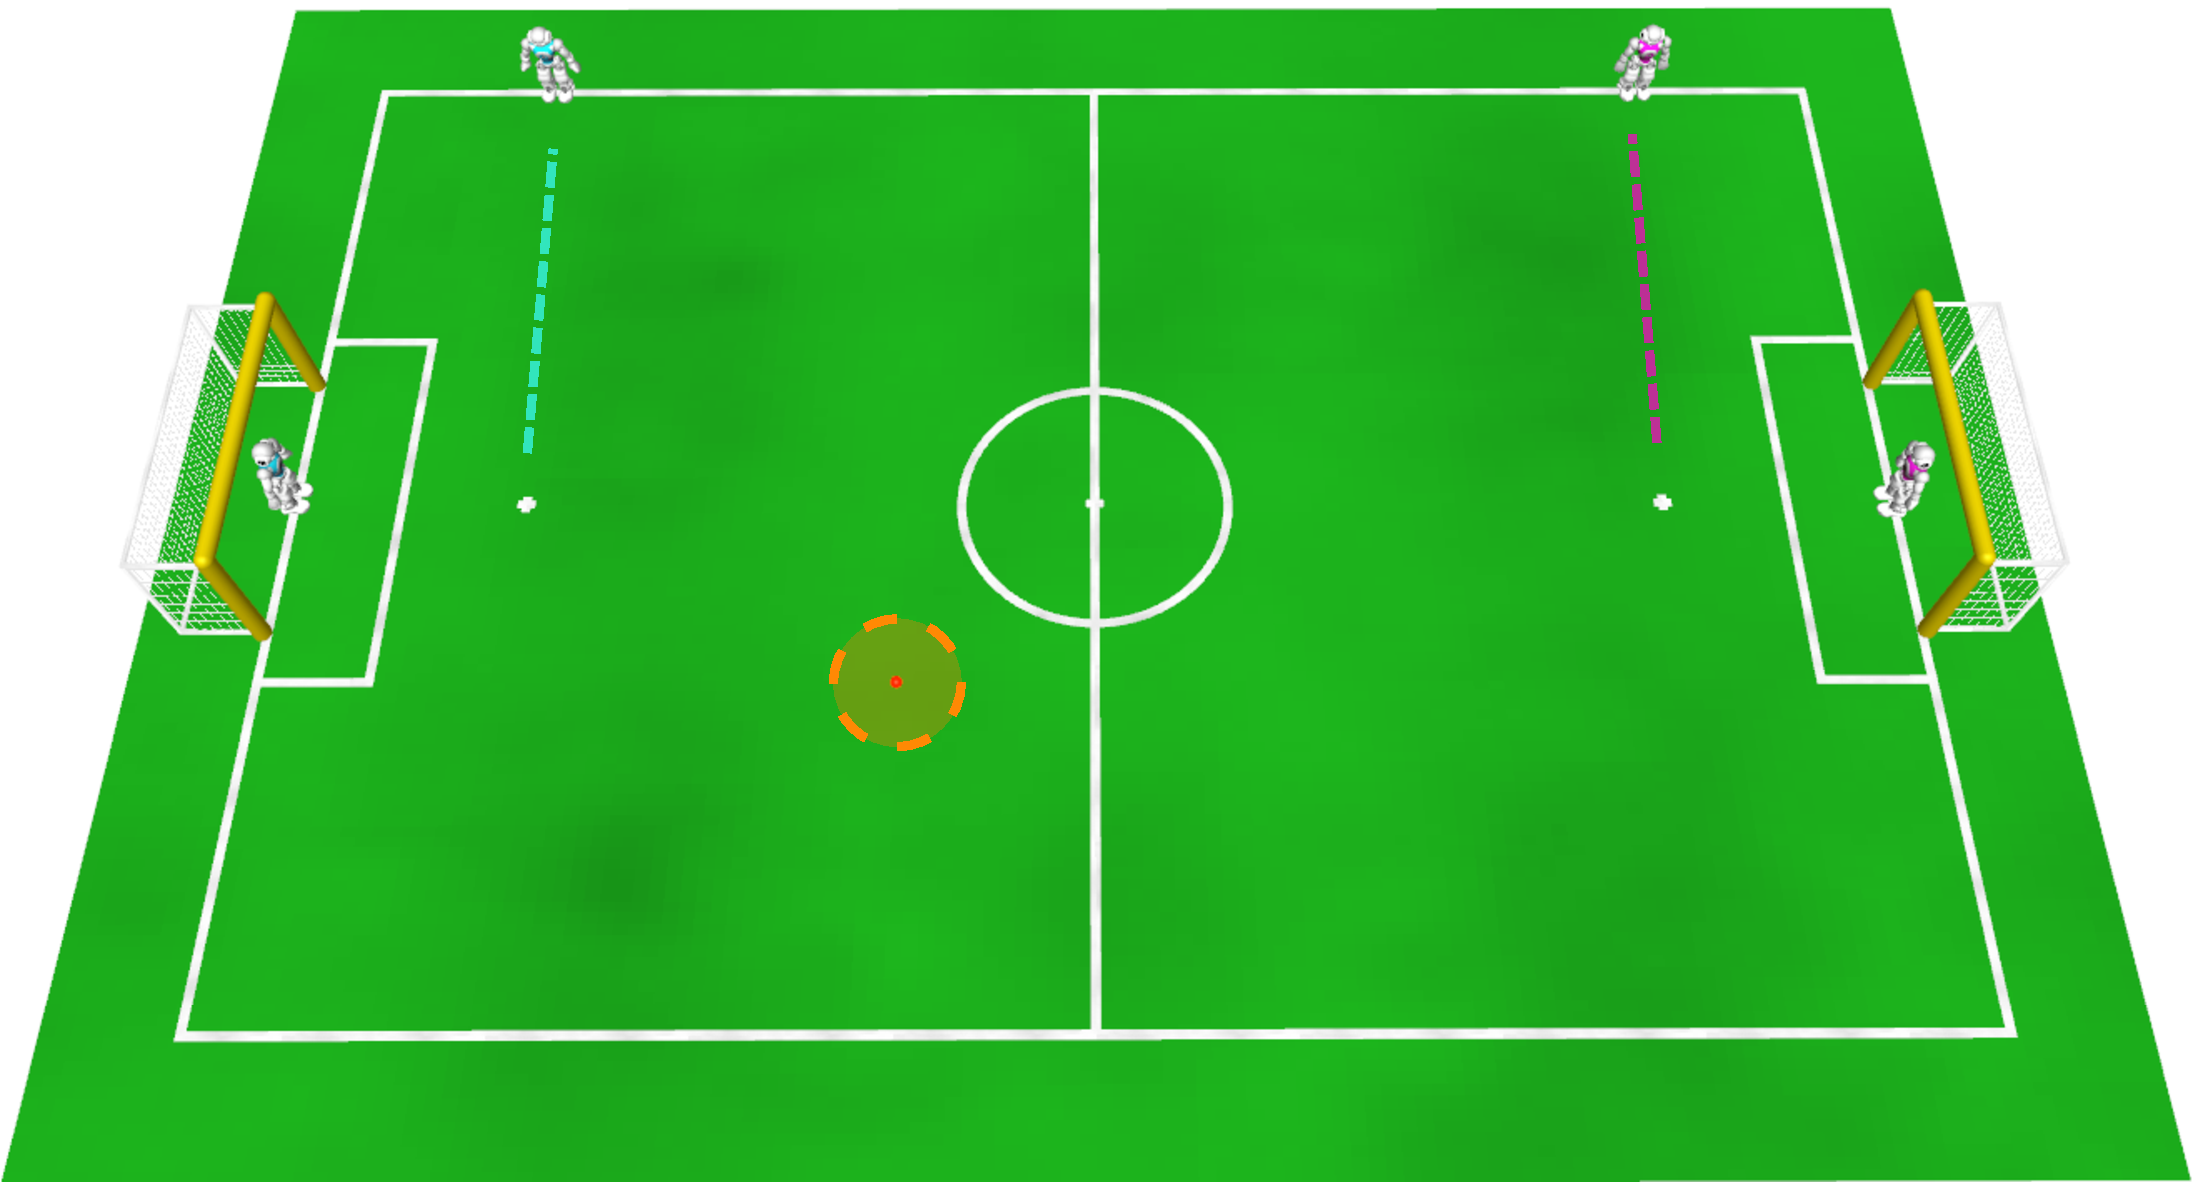
\includegraphics[width=\columnwidth]{figs/penalty_re-entry_points.pdf}}
\caption{For robots coming back from a standard removal penalty, re-entry points lie in their own half, on the sideline on the side away from the ball.}
\label{fig:penalty_re-entry_points}
\end{figure}

When the robot is on the field again, the operator of the GameController will send the \emph{playing} signal to it. If the wireless is not working, the assistant referee who placed the robot back on the field has to bring it into the \emph{playing} state again.

\subsection{Manual Interaction by Team Members}

Manual interaction with the robots, either directly or via some communications mechanism, is not permitted. Team members can only touch one of their robots when an assistant referee hands it over to them after a ``Request for Pick-up''.

\subsection{Kick-off Shot}
\label{sec:kick-off_shot}

A ``kick-off shot'' --- a shot taken by any of the two teams after a kick-off before the entire ball has left the center circle, including the boundary line --- can usually not score a goal. There are two instances in which a ``kick-off shot'' may score: (1) if the ball touches a teammate of the kicking robot outside the center circle before entering the goal and (2) if a team scores an own goal.
 
Otherwise, if a kick-off shot enters the goal (either directly or via contact with an opponent), no goal will be scored and the standard removal penalty will be applied to the kicking robot. The ball will be put back to the place from which it was kicked. At this point, either team may attempt to shoot the ball on goal.


\subsection{Ball Holding}
\label{sec:ball_holding}

The goal keeper is allowed to hold the ball for up to 10 seconds as long as it has one foot inside in its own penalty area.  In all other cases (except those noted in Section \ref{sec:situations_no_ball_holding}), robots are allowed to hold the ball for up to 3 seconds. Holding the ball for longer than this is ``Ball Holding'' and is not allowed.

A robot which does not leave enough open space around the ball will be penalized as ``Ball Holding'' if that situation continues more than 3 seconds. The occupation of the ball is judged using the convex hull of the projection of the robot's body onto the ground. ``Enough open space'' means that at least the half of the ball is not covered by the convex hull. It is not important whether the robot actually touches the ball.

\begin{figure}[t]
\centerline{\begin{tabular}{ll}
a) & b) \\
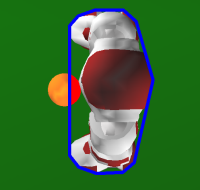
\includegraphics[scale=0.7]{figs/holding1} &
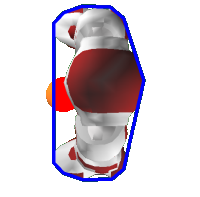
\includegraphics[scale=0.7]{figs/holding4}
\end{tabular}}

\caption{Examples for ``Ball Holding''. The black circle is the ball, the blue polygon visualizes the convex hull of the robot's projection onto the ground and the red area shows the occupied portion of the ball. Situations a) is legal, whereas b) violates the rule.}
\label{fig:holding}
\end{figure}

Intentional continual holding is prohibited even if each individual holding time does not continue for up to the time limit. In general, robots should release the ball for approximately as long as they were holding it to reset the clock. Without a sufficient release, the continual holding is regarded as a continuous hold from the very beginning and the holding rule is strictly applied. The violation of this rule will result in the standard removal penalty (see Section~\ref{sec:removal_penalty} for details). The ball should be removed from the possession of the robot and placed where the foul occurred. If the robot that held the ball has moved the ball before the robot can be removed, the ball shall be replaced where the foul occurred.

\paragraph{Example.} A robot holds the ball and before the referees
can remove the robot, it shoots the ball into the goal. The goal
will not be counted and the ball will be replaced where the robot
held the ball.

\subsubsection{Exceptions to the Ball Holding Rules}
\label{sec:situations_no_ball_holding}

The following define situations where ball holding does not apply:

\begin{enumerate}
	\item Ball holding may not occur when the ball becomes stuck between a robot's legs.  In such a situation, the head referee should call `clear ball' and an assistant referee should remove the ball and place the ball approximately where it was before it became stuck.
	\item Ball holding may not occur when a robot falls on a ball.  The robot will either get-up and hence free the ball, or the robot should be removed under the Fallen Robot rule.
\end{enumerate}


\subsection{Fallen or Inactive Robots}
\label{sec:fallenrobots}

If a robot falls during the game, it should start executing a getup action within 5 seconds. If it does not commence a get up action within 5 seconds, it will be removed as per the standard removal penalty. A robot which is unable to autonomously stand up within 20 seconds after a fall will be removed and subject to the standard penalty. The goal keeper, inside its own penalty area, is the only robot permitted to `dive' (that is deliberately fall in a way that might cause its torso, arms or hands) to intercept the ball. In all other cases, the robot should be programmed to attempt to remain upright -- that is, supported by its feet.

A robot that has ceased activity for 10 seconds or has turned off will be removed by the referees and is subject to the standard removal penalty. A robot is active if it performs at least one of the following:

\begin{enumerate}

\item The robot walks in any direction, or turns.

\item The robot searches for the ball, or is looking at the ball.

\end{enumerate}

\paragraph{Note:} The intention of this rule is not to penalize robots simply for being stationary -- provided they are not `asleep' and have not `crashed'.

\subsection{Player Stance}
\label{sec:player_stance}

Robots are not allowed to stay in a stance that is wider than the width of the robot's shoulders for more than 5 seconds. The robot is allowed to go into a wide stance as long as it comes back to a normal stance within 5 seconds. Staying in a wide stance for longer than 5 seconds will result in the standard penalty. If the robot has fallen down, it must start getting up within 5 seconds. 

\subsection{Coach Motion}
\label{sec:coach_motion}

The coach robot has to remain seated during the whole game, it is only allowed to move its arms and head. If the robot leaves its seating position, it will be disqualified for the remainder of the game and has to leave its position on the table. Technically, this is handled as a Request for Pick-Up
(\cf Section \ref{sec:request_for_pickup}) but without the possibility to reenter the game.

\subsection{Player Pushing}
\label{sec:player_pushing}

% basic definition of pushing
\emph{Pushing} is a forceful contact with another robot, i.e., enough to destabilize it, and is not allowed. In the following, the cases when pushing occurs as well as exceptions are specified in more detail.

If the ball moves significantly as the result of pushing, then it should be replaced to where it was at the time of the infringement.

\subsubsection{Exceptions to the Pushing Rules}
\label{sec:situations_no_pushing}

The following define situations where pushing does not apply:

\begin{enumerate}
	\item Pushing may occur \textbf{only} between players of different teams.
	\item A stationary robot cannot be penalized for pushing, including a robot that is kicking, provided that the ball was close enough where a kick could have succeeded at the start of the kick motion.
	\item A robot currently getting up cannot be penalized for pushing.
	\item The goal keeper cannot be penalized for pushing while looking at or chasing the ball in it's own penalty area.
	\item Front to front contact between robots with the ball between them does not constitute pushing.
	\item Any robot proceeding to the ball whose side (\ie arm, shoulder etc.) makes contact with another robot cannot be called for pushing. Even if the second robot is not proceeding to the ball.
	\item A robot pushed by another robot can not simultaneously be called for pushing itself.
\end{enumerate}

\subsubsection{Contact between standing/walking Robots}
\label{sec:pushing_contact}

The following forms of contact are considered pushing contacts except for the conditions in Section~\ref{sec:situations_no_pushing}:
\begin{enumerate}
	\item Any form of forceful contact that significantly destabilizes a robot, such that walking and/or kicking is impeded. Examples for forceful contacts include falling into another robot or walking carelessly into another robot at significant speed.
	\item Walking into another robot for 2 seconds (even a fallen or getting up robot), even if the `force to push' is minimal.
\end{enumerate}

\subsubsection{Contact Between More Than 2 Robots}
\label{sec:pushing_several_robots}

Pushing should be called in the same way when multiple robots are in contact. The robot that is pushing will be called for a penalty regardless of how many robots of either team are in the area. This is to ensure that the team that is pushing is called for the penalty. If any of the exceptions apply to a robot in the group, that robot cannot be called for pushing.

\subsection{Playing with Arms/Hands}
\label{sec:hand_ball}

A field player (including a defender) or a goal keeper outside its own penalty box that touches the ball with its arms/hands will be subject to the standard removal penalty and the ball is to be replaced at the point where it contacted the arms/hands of the offending robot.  If an own goal is scored as a result, the goal should count and the player should not be penalized.

\subsection{Damage to the Field}
\label{sec:damage}
A robot that damages the field will be removed from the field for the remainder of the game. Similarly, a robot that poses a threat to spectator safety will also be removed from the field for the remainder of the game.

\subsection{Leaving the Field}
\label{sec:leaving_field}

A robot that intends to leave the \TotalWidth $\times$ \TotalLength carpeted area will be subject to the standard removal penalty (see
Section~\ref{sec:removal_penalty}). This penalty can already be called after a robot leaves the 6~m $\times$ 9~m playing field if the robot appears to be ``lost''.

In addition, 
\begin{itemize}
\item a robot that walks into the goal net for more than 5 seconds as well as 
\item a robot whose fingers become entangled in the net (without any time constraint)
\end{itemize}
will also be subject to the standard removal penalty.

\subsection{Illegal Defender}
\label{sec:illegal_defender}

Only two players can be within a team's penalty area at the same time. A robot is within the penalty area if any part of its body is touching the ground inside the penalty box or touching one of its lines.  When any additional players (whether field player or goalkeeper) enter the area, they will be subject to the standard removal penalty (see Section~\ref{sec:removal_penalty}). This is called the ``Illegal Defender Rule''. Note that if an operational defender is pushed into the penalty area by an opponent, this robot will not be subject to removal unless it fails to exit the area within 5 seconds (or 5 seconds of getting up if the pushing led to falling).

If an illegal defender kicks an own goal, the goal is scored for the opponent. If there is any doubt about whether a goal should count (e.g. the illegal defender infraction is called, but the robot scores the own goal immediately afterwards, before it is removed) then the decision shall be against the infringing robot.

The ``Illegal Defender'' penalty is also applied to defensive players that enter the center circle after a kick-off before the ball is in play (\cf Section~\ref{sec:kick-off}).

\subsection{Jamming}
\label{sec:jamming}
During the match any robot shall never jam the communication and the sensor systems of the opponents:

\begin{description}

\item[Wireless communication.] As specified in Sect. \ref{sec:wireless}, each robot is only allowed to send a limited number of UDP messages that have to comply with a predefined format. If a robot uses a different protocol or sends too many messages over a couple of seconds in a game, it will be disqualified for that game. If a teams violates this rule in multiple games, disqualification from the tournament (including technical challenges as well as the drop-in competition) as well as an entry in the penalty list will be the consequence. Except for the wireless cards and the access points provided by the organizers of the competition, nobody close to the field is allowed using 2.4~GHz radio equipment (including cellular phones and/or Bluetooth devices).

\item[Acoustic communication.] If acoustic communication is used by both teams, they shall negotiate before the match how they can reduce interference. If only one team uses acoustic communication, the robots of the other team shall avoid producing any sound. In addition, both the teams and the audience shall avoid intentionally confusing the robots by producing similar sounds to those used for communication.

\item[Infrared communication.] If infrared communication is used by both teams, they shall negotiate before the match how they can reduce interference (if at all). Both the teams and the audience shall avoid confusing the robots by producing similar infrared signals to those used for communication.

\item[Visual perception.] The use of flashlights is not allowed during the games.  However, flash photography from the audience is allowable as long as the head referee believes the purpose of the flash is not to jam any of the robots.

\end{description}


\newpage


\section{Judgment}

The referees are the only persons that are allowed on the carpeted area (\ie the field and the border area).

\subsection{Head Referee}
\label{sec:head_referee}
The head referee signals game starts, restarts, and the case of \emph{game stuck} by a single whistle. In general, the head referee first whistles and then announces the reason for the whistle. The only exception is the case of the kick-off, in which the reason for the whistle is obvious. The whistle defines the point in time at which the decision is made. In case of a local or global game stuck, this is also announced verbally. By two whistles, the head referee terminates the first half; by three whistles he terminates the second half, \ie the whole game.  Goals should be indicated verbally and by the head referee pointing with one arm towards the center of the field.

In the penalty kick shoot-out, the head referee keeps the time.

Any decision of the head referee is valid. There is no discussion about decisions during the game, neither between the assistant referees and the head referee, nor between the audience or the teams and the head referee. The main referee's decision is final and can not be changed afterwards by video proof.

\subsection{Assistant Referees}
\label{sec:assist_referee}
The two assistant referees handle the robots and the ball. They start the robots if the wireless is not working, they move the robots manually to legal kick-off positions, they take the robots out when they are penalized, and they put the robots in again. If a team requests to pick up a robot, an assistant referee will pick it up and give it to one of the team members once the head referee approves. An assistant referee will also put the robot back on the field. An assistant referee will also replace the ball when it goes off the field or becomes stuck between a players feet.  In addition, the assistant referees can indicate violations against the rules committed by robots to the head referee, so that the head referee can decide whether to penalize a certain robot or not. Assistant referees should only enter the field to execute a decision made by the main referee. They should not prevent robots from falling during the game.

\subsection{Operator of the GameController}
\label{sec:gameControllerOp}
The operator of the GameController sits at a PC outside the playing area. He or she will signal any change in the game state to the robots via the wireless as they are announced by the head referee. Please note that for the kick-off, the moment of whistling is determining, not the verbal announcement of the head referee. He or she will also inform the assistant referees when a timed penalty is over and a robot has to be placed back on the field. He or she should announce to the head referee when the ball is in play on kick-off (if this occurs because 10 seconds have elapsed in the playing state) by stating ``Ball in Play''. The operator is also responsible for keeping the time of each half, \ie, he or she stops the clock after a goal or game stuck, and continues it at the kick-off\footnote{The clock may not be stopped during the preliminaries.}.  The operator should count aloud the remaining seconds in a half once the time remaining is 5 seconds or less.

\subsection{Referees During the Match}

The head referee and the assistant referees should wear clothing and socks \emph{of black or dark blue color} (blue jeans are acceptable) and avoid reserved colors for the ball, the goals, and player markings in their clothing. They may enter the field in particular situations, \eg, to remove a robot when applying a penalty. They should avoid interfering with the robots as much as possible.

\subsection{A Remark on Artificial Landmarks}
\label{sec:judgment:landmarks}

The head referee may decide at any point before or during a game to relocate any objects around the field, or direct persons to another position around the field.

The intent of using same-colored goals is to remove artificial landmarks.
Robots should be able to localize with the SPL field and its ``normal'' surroundings.
Introducing new team-specific artificial landmarks is against the spirit and intention of the league's progress.
The application of this rule needs to be well considered and should be reserved for situations which seem constructed by one team or another, but will ultimately be the head referee's decision alone.


\newpage


\appendix
\section{The Official RoboCup Competition Rules}
\label{sec:comRules}
This section contains rules that are not directly relevant for games and that may not apply at local opens.  However, these rules will be upheld at the yearly international RoboCup competition.

\subsection{Game Structure}

The clock stops during stoppages of play (such as ready and set state after goals) from the quarter-finals onward.  In round robin pool play, a game can finish in a draw as no penalty shoot-out will follow. In the intermediate round, quarter finals, semi finals, 3rd place or final, a game that ends in a draw will be followed by a penalty shoot-out (see Section~\ref{sec:penalty_shoot-out}).

\subsection{Winner and Rankings}
\label{sec:rankings}

The team which scored more goals than the other is the winner of the match. If the two teams scored the same number of goals, the game will be a draw. The draw will follow the same system defined in Section~\ref{sec:game_struct}. Total (and final) standings will be decided on points as follows (the points will be given based on the result of each game):

\makebox[\columnwidth]{ \hfill Win = 3 pts\hfill Draw = 1 pt \hfill
Lose = 0 pts\hfill }

If a team's obtained points is the same as another team's after a round of pool play is complete, the following evaluations will be applied in order to qualify the finalists.

\begin{enumerate}

\item The points obtained

\item The difference between goals for and goals against per game

\item The average goals for per game

\item Game result between the teams directly

\end{enumerate}

\subsection{Champions cup and Challenge shield}
\label{sec:twoCompetitions}
In order to provide better matched games for teams of all abilities the RoboCup Standard Platform League shall be divided into two separate competitions: the Champions cup for the strongest teams and the Challenge shield for all other teams. Final assignment of teams to each competition occurs at RoboCup based on initial game performance.

It is proposed that the SPL will qualify 24 teams, but if the numbers qualified change the numbers in the following may be altered slightly.

All teams who qualify for participation in the RoboCup SPL are ranked on the basis of their previous year's RoboCup result in accordance with the ranking described in \ref{sec:rankings}. (New teams will be ranked equally below all previously competing teams. Teams that participated previously but did not participate in the previous year will be ranked above new teams but below teams that competed in the previous year.) The top 12 teams (by rank) will be Champions cup candidates and the remaining teams will be Challenge shield candidates.

All Champions cup candidates play a single qualifier round robin stage comprising 4 groups of 3 teams each. All Challenge shield candidates play a similar qualifier round robin stage also consisting of 4 groups of 3 teams each. Each Champions cup qualifier group will consist of one team ranked 1-4, one team ranked 5-8, and one team ranked 9-12. Each of the teams ranked 13-16 will be placed in a different Challenge shield group. Remaining Challenge shield qualifier group places will be filled by random selection from teams ranked 17-24.

The top 2 teams in each Champions cup qualifier group proceed automatically to the Champions cup proper. Similarly the lower 2 teams in each Challenge shield qualifier group proceed automatically to the Challenge shield. The 4 remaining Champions cup candidates (losers in each group) play the remaining Challenge shield candidates (winners in each group) and the winners of these games go the Champions cup while the losers go to the Challenge shield. Thereafter, the Champions cup and Challenge shield competitions shall proceed independently of each other and each will normally consist of a round robin stage followed by a knockout competition.


\subsection{Selection of the Referees}
\label{sec:refSelection}
During pool play, the games will be refereed by members of teams from a different pool.  Each team has to referee a number of games --- a refereeing schedule will be released prior to the competition. For each of the games, a team can either provide the head referee and the operator of the GameController, or the two assistant referees.  Note that the head referee and the GameController should always be from the same team.  The two teams assigned to referee a game shall decide among themselves which roles each team will fulfill.  Referees must have good knowledge of the rules as applied in the tournament, and the operator of the GameController must be experienced in using that software. Both referees and the GameController are expected to have studied for, taken, and passed an online rule test which will be available before RoboCup.  Referees and the GameController should be selected among the more senior members of a team, and preferably have prior experience with games in the RoboCup Standard Platform league.

In each game, each of the teams playing shall be able to veto one and only one eligible referee with no reason required.

\subsection{Subsequent Year Pre-Qualification Procedure}
\label{sec:preQual}
Teams may become pre-qualified for the subsequent year's team competition by reaching the quarter-finals in the team competition.

However, pre-qualified teams must do all of the following in order to remain pre-qualified:
\begin{itemize}
\item Post in a publicly available location a team research report describing their work for the 2017 competition
\item Publicly release code from that year's codebase, either in the form of a complete release (perhaps without behavior) or limited libraries.  This release must be documented and coded in a way where it can be used by others.
\item Submit a shortened application as required by the call for participation for the subsequent year's competition
\end{itemize}

\subsection{Penalty for Failing to Referee when Assigned}
\label{sec:refPenalty}
A schedule will be released regarding the games for which each team is required to provide two referees.  These referees should report to the field on which the game they are to referee is to be played at least five minutes before the game is scheduled to start.

Each time a team fails to provide two referees for a game in which they are scheduled to provide referees, it will be noted by the organizing committee.  Failing to provide referees when assigned is a serious offense that will not only cost you pre-qualification for the subsequent year if your team has otherwise earned pre-qualification, but will also severely effect your team's chances of being accepted the following year.

A team may swap refereeing duties with another team, but the team listed on the referee schedule will be held accountable if referees fail to appear for a game they are scheduled to referee.

The requirement to referee may be an extreme hardship for extremely small teams.  If a team believes providing two referees for games will be an extreme hardship, they must send an email explaining their situation to the Organizing Committee and Technical Committee at least two weeks before the first set up day of the competition.  The Organizing and Technical Committees will then consider the request and attempt to find an acceptable solution.

\section{Mixed Team Tournament}
\label{sec:mixedTeamTournament}
This section contains all rules regarding the mixed teams tournament, which will replace the drop-in player competition. In the first years of the tournament, random teams will not be mixed together and only a limited number of teams will participate.  In future years of the tournament, we hope that teams would develop infrastructures that could allow the mixed team compositions to change throughout the tournament.

For the 2017 tournament, pairs of teams will announce their partnership as part of the answer to the official call for application. As part of the application, potential team pairs should announce the name of the second team, the mixed team name, and their proposed jersey color.

\subsection{Limitations}
In 2017, the tournament will be limited to four mixed teams. Both teams comprising a mixed team should run their own codebase, but are encouraged to develop a layer for interoperability which could later be used to form mixed teams with other teams. 

\subsection{Process of the Tournament}
Depending on logistical issues, the tournament will be played either 10 vs 10 on a MSL field or 6 vs 6 on a SPL field. We will announce which type of field will be used by the end of March 2017. Besides the field size and number of players, all other normal SPL rules apply. 

For the 2017 tournament, there will be eight games in total: a round robin round with 6 games, a 3rd place game, and a championship game.  Hence, each mixed team would play a total of 4 games in the mixed team tournament.

\newpage

\section{Changes From 2016}
This is a brief list of rule changes from 2016 to 2017.

\subsection*{Setup of the Environment}
\begin{itemize}
	\item The field surface is 8mm artificial turf. (Section \ref{sec:field_dim})
	\item The lighting conditions shall favour window lighting where possible and will allow for uneven lighting (Section \ref{sec:lightConditions})
\end{itemize}

\subsection*{Robot Players}
\begin{itemize}
	\item Plating on NAO robots can be gray, red, blue, or orange. (Section \ref{sec:hardware})
	\item The coaching robot can be placed anywhere on the sideline tables. (Section \ref{sec:coaching_robot})
	\item Relax restrictions on how much and how often the coaching robot can send packets.  Also remove restrictions on data formatting. (Section \ref{sec:wireless})
\end{itemize}

\subsection*{Game Process}
\begin{itemize}
	\item The penalty shootout procedure has been streamlined by reducing the number of penalties and the time limit for each penalty shot. Robots and replacements must now be handed over at the start of the penalty shootout. (Section \ref{sec:penalty_shoot-out})
\end{itemize}

\subsection*{Drop-in Player Competition}
Deleted

\subsection*{Outdoor Competition}
Deleted

\subsection*{The Official RoboCup Competition Rules}
\begin{itemize}
	\item Introduce the division of the SPL into two competitions: the Champions cup and the Challenge shield. (Section \ref{sec:twoCompetitions})
\end{itemize}

\subsection*{Mixed Team Tournament}
\begin{itemize}
	\item Introduced the new mixed teams tournament. (Section \ref{sec:mixedTeamTournament})
\end{itemize}
\end{document}

